\documentclass[12pt,a4paper]{report}

% ---------- kodowanie i język ----------
\usepackage[T1]{fontenc}
\usepackage[utf8]{inputenc}
\usepackage[polish]{babel}
\usepackage{lmodern}
\usepackage{csquotes}

% ---------- matematyka ----------
\usepackage{amsmath,amssymb}

% ---------- układ strony ----------
\usepackage[a4paper,left=3cm,right=3cm,top=2.7cm,bottom=2.7cm]{geometry}
\usepackage{setspace}
\onehalfspacing
\tolerance=2000
\emergencystretch=3em

% ---------- grafika i tabele ----------
\usepackage{graphicx}
\graphicspath{{figures/}}
\usepackage{booktabs}
\usepackage{longtable}
\usepackage{float}
\usepackage{caption}
\usepackage{subcaption}
\captionsetup{font=small,labelfont=bf}

% ---------- kolory, listingi ----------
\usepackage{xcolor}
\definecolor{codebg}{RGB}{247,247,247}
\definecolor{codekw}{RGB}{44,62,80}
\definecolor{codecm}{RGB}{39,110,60}
\definecolor{codestr}{RGB}{192,57,43}
\definecolor{codeln}{RGB}{150,150,150}
\usepackage{listings}
\lstdefinelanguage{Chapel}{
  keywords={proc,const,config,var,use,forall,coforall,for,do,on,if,then,else,return,
            in,ref,new,writeln,writef,record,class,param,type,inout,out,begin,serial,
            local,while,when,select,module,import,require,extern,override,throws,try},
  keywordstyle=\color{codekw}\bfseries,
  comment=[l]{//}, morecomment=[s]{/*}{*/},
  commentstyle=\color{codecm}\itshape,
  string=[b]", stringstyle=\color{codestr},
  sensitive=true,
}
\lstset{
  basicstyle=\ttfamily\footnotesize,
  backgroundcolor=\color{codebg},
  numbers=left, numberstyle=\tiny\color{codeln}, numbersep=7pt,
  frame=single, rulecolor=\color{codeln!60},
  breaklines=true, showstringspaces=false,
  captionpos=b, aboveskip=1.1em, belowskip=0.6em,
  literate={ą}{{\k a}}1 {ę}{{\k e}}1 {ó}{{\'o}}1 {ł}{{\l}}1 {ż}{{\.z}}1
           {ź}{{\'z}}1 {ć}{{\'c}}1 {ś}{{\'s}}1 {ń}{{\'n}}1
           {Ą}{{\k A}}1 {Ę}{{\k E}}1 {Ó}{{\'O}}1 {Ł}{{\L}}1 {Ż}{{\.Z}}1,
}
\lstdefinestyle{bash}{language=bash,keywordstyle=\color{codekw}\bfseries,
  commentstyle=\color{codecm}\itshape,morecomment=[l]{\#}}
% ---- nie dziel listingów między strony: całe środowisko w nierozrywalnym boksie ----
% (jeśli listing nie mieści się na dole strony, przechodzi w całości na następną)
\AddToHook{env/lstlisting/before}{\par\medskip\noindent\begin{minipage}{\linewidth}}
\AddToHook{env/lstlisting/after}{\end{minipage}\par\medskip}

% ---------- diagramy ----------
\usepackage{tikz}
\usetikzlibrary{positioning,arrows.meta,calc,3d,fit,backgrounds,shapes.geometric}

% ---------- odnośniki ----------
\usepackage[hidelinks,pdfusetitle]{hyperref}

% ============================================================
% Lekkie namiastki pakietów niedostępnych w tym środowisku TeX
% (siunitx, cleveref, emptypage, multirow) — realizowane na xstring.
% ============================================================
\usepackage{xstring}
\makeatletter
% ---- przecinek dziesiętny i jednostki (namiastka siunitx) ----
\DeclareRobustCommand{\deccomma}[1]{\StrSubstitute{#1}{.}{,}}
\DeclareRobustCommand{\num}[1]{\ifmmode\text{\deccomma{#1}}\else\deccomma{#1}\fi}
\DeclareRobustCommand{\si}[1]{#1}
\DeclareRobustCommand{\SI}[2]{\num{#1}\,{#2}}
\DeclareRobustCommand{\numrange}[2]{\num{#1}--\num{#2}}
\DeclareRobustCommand{\SIrange}[3]{\num{#1}--\num{#2}\,{#3}}
\providecommand{\giga}{G}\providecommand{\mega}{M}\providecommand{\kilo}{k}
\providecommand{\milli}{m}\providecommand{\micro}{\ensuremath{\mu}}
\providecommand{\bit}{b}\providecommand{\byte}{B}\providecommand{\second}{s}
\providecommand{\metre}{m}\providecommand{\meter}{m}\providecommand{\hertz}{Hz}
\providecommand{\watt}{W}\providecommand{\joule}{J}\providecommand{\gram}{g}
\providecommand{\ampere}{A}\providecommand{\per}{/}
\providecommand{\squared}{\ensuremath{^{2}}}\providecommand{\cubed}{\ensuremath{^{3}}}
\providecommand{\percent}{\%}\providecommand{\degree}{\ensuremath{^\circ}}
\providecommand{\celsius}{\ensuremath{^\circ}C}\providecommand{\kelvin}{K}
\providecommand{\ohm}{\ensuremath{\Omega}}
% ---- odsyłacze (namiastka cleveref, polskie nazwy; parsowanie prefiksu etykiety) ----
\@namedef{crlc@ch}{rozdz.}\@namedef{crlc@sec}{podrozdz.}\@namedef{crlc@fig}{rys.}%
\@namedef{crlc@tab}{tab.}\@namedef{crlc@lst}{listing}\@namedef{crlc@eq}{równ.}
\@namedef{cruc@ch}{Rozdział}\@namedef{cruc@sec}{Podrozdział}\@namedef{cruc@fig}{Rysunek}%
\@namedef{cruc@tab}{Tabela}\@namedef{cruc@lst}{Listing}\@namedef{cruc@eq}{Równanie}
\def\cref@get#1:#2\@nil{#1}
\newcommand{\cref@do}[2]{%
  \edef\@crefp{\cref@get#2:\@nil}%
  \@ifundefined{#1@\@crefp}{poz.}{\csname #1@\@crefp\endcsname}~\ref{#2}}
\DeclareRobustCommand{\cref}[1]{\cref@do{crlc}{#1}}
\DeclareRobustCommand{\Cref}[1]{\cref@do{cruc}{#1}}
% ---- multirow (nieużywane, na wszelki wypadek) ----
\providecommand{\multirow}[3]{#3}
\makeatother

% ---------- meta ----------
\newcommand{\thesistitle}{Programowanie równoległe w~języku Chapel na~przykładzie problemu rozchodzenia się ciepła}
\newcommand{\thesisauthor}{Szymon Orzechowski}
\newcommand{\thesissupervisor}{[promotor do uzupełnienia]}
\newcommand{\thesisuniversity}{[uczelnia / wydział do uzupełnienia]}
\newcommand{\thesisyear}{2026}

\title{\thesistitle}
\author{\thesisauthor}
\date{\thesisyear}

\begin{document}

% ======================= STRONA TYTUŁOWA =======================
\begin{titlepage}
\centering
\vspace*{1.5cm}
{\large \thesisuniversity\par}
\vspace{2.5cm}
{\LARGE\bfseries Praca magisterska\par}
\vspace{1.2cm}
{\Large\bfseries \thesistitle \par}
\vspace{2.5cm}
\begin{flushright}
{\large \thesisauthor\par}
\vspace{0.4cm}
{\normalsize Promotor: \thesissupervisor\par}
\end{flushright}
\vfill
{\large \thesisuniversity{} --- \thesisyear\par}
\end{titlepage}
\cleardoublepage

% ======================= SPIS TREŚCI =======================
\tableofcontents

% ======================= ROZDZIAŁY =======================
\chapter*{Wstęp}
\addcontentsline{toc}{chapter}{Wstęp}
\markboth{Wstęp}{Wstęp}
\label{ch:wstep}

Symulacje zjawisk opisanych równaniami różniczkowymi cząstkowymi należą do najczęściej
spotykanych zadań obliczeniowych w~nauce i~inżynierii. Wśród nich szczególne miejsce zajmują
obliczenia \emph{stencilowe}, czyli takie, w~których nowa wartość w~każdym punkcie siatki jest
funkcją wartości z punktów sąsiadujących.

Trójwymiarowe równanie przewodnictwa ciepła jest tradycyjnym przykładem takiego problemu.
Jego jawna dyskretyzacja różnicowa posiada niską intensywność arytmetyczną
oraz konieczność wymiany danych brzegowych między częściami dziedziny w~każdym kroku
czasowym~\cite{datta-stencil} co sprawia, że obliczenia stencilowe
są trudne do zrównoleglenia. Program symulujący to równanie nadaje się dobrze do badania granic skalowalności, ponieważ jego prosty wzorzec komunikacji, ograniczony do wymiany z~najbliższymi sąsiadami,
przy licznych węzłach i~tak obciąża współdzielone łącze sieciowe,
co ujawnia ograniczenia komunikacyjne klastra.

Programowanie równoległe tradycyjnie realizuje się za pomocą interfejsu
przekazywania komunikatów MPI (ang.~\emph{Message Passing Interface}), zyskując wysoką wydajność kosztem znacznej złożoności kodu, gdyż
programista jawnie zarządza podziałem danych, buforami wymiany oraz synchronizacją~\cite{mpi-standard}. Alternatywę
oferują języki i~biblioteki oparte na modelu \emph{PGAS} (ang.\ \emph{Partitioned Global Address
Space})~\cite{pgas}. Język Chapel,
rozwijany pierwotnie przez firmę Cray, jest
jednym z~bardziej rozwiniętych języków w~tej grupie~\cite{chapel-overview}. Umożliwia zapisywanie obliczeń
rozproszonych w~notacji zbliżonej do sekwencyjnej, z~globalnym widokiem tablic, wysokopoziomowymi
iteratorami równoległymi i~gotowymi rozkładami dziedzin. Szczegóły komunikacji pozostawia
warstwie wykonawczej, opartej na bibliotece GASNet.

Zbliżoną tematykę podjęto w~pracy współautorskiej
poświęconej równoległej symulacji dwuwymiarowego przewodnictwa ciepła na~klastrze Raspberry~Pi
oraz porównaniu implementacji w~językach Chapel, C\# i~Julia~\cite{falkowski2026parallel}, podczas
gdy niniejsza praca obejmuje przypadek trójwymiarowy na~klastrze Pionier.

Celem niniejszej pracy było zaprojektowanie, zaimplementowanie i~wdrożenie na~klastrze
programu symulującego równanie przewodnictwa ciepła w~Chapel oraz
analiza jego poprawności i~skalowalności.

\chapter{Problem i wykorzystane technologie}
\label{ch:problem}

\section{Równanie ciepła i metoda różnic skończonych}
\label{sec:heat-fdm}

\subsection{Model fizyczny}

Rozważanym zjawiskiem fizycznym jest dyfuzja ciepła w~jednorodnym, izotropowym
ośrodku wypełniającym sześcian jednostkowy \(\Omega = [0,1]^3\). Pole skalarne
\(u(\mathbf{x},t)\) opisuje temperaturę w~punkcie \(\mathbf{x}=(x,y,z)\in\Omega\)
w~chwili \(t\ge 0\). Ewolucję tego pola opisuje równanie różniczkowe
cząstkowe znane jako równanie przewodnictwa ciepła, zwane też równaniem dyfuzji:
\begin{equation}
  \frac{\partial u}{\partial t} \;=\; \alpha\,\nabla^2 u
  \;=\; \alpha\!\left(
    \frac{\partial^2 u}{\partial x^2}
    + \frac{\partial^2 u}{\partial y^2}
    + \frac{\partial^2 u}{\partial z^2}
  \right),
  \label{eq:heat3d}
\end{equation}
gdzie \(\nabla^2\) oznacza operator Laplace'a, natomiast
\(\alpha>0\) to współczynnik dyfuzyjności cieplnej (ang.\ \emph{thermal
diffusivity}), wyrażony w~jednostkach \si{\metre\squared\per\second}. Wielkość
\(\alpha\) łączy przewodność cieplną ośrodka z~jego pojemnością cieplną i~gęstością;
im większa jej wartość, tym szybciej lokalne różnice temperatury ulegają
wygładzeniu. W~zaimplementowanym programie przyjęto bezwymiarową wartość
\(\alpha = \num{0.25}\) jako parametr konfiguracyjny.

\subsection{Warunki początkowe i brzegowe}

Rozwiązanie równania~\eqref{eq:heat3d} jest jednoznaczne dopiero po~zadaniu
warunku początkowego oraz warunków brzegowych. W~zaimplementowanym rozwiązaniu
warunek początkowy przyjmuje jednorodne pole \(u(\mathbf{x},0)=1\) w~całej
dziedzinie, w~którym umieszczono nagrzaną warstwę 
o~grubości \texttt{hotThickness} płaszczyzn siatki przylegających do~ściany
\(y=0\), o~podwyższonej wartości \(u=2\). Warstwa ta modeluje gorącą ścianę,
od~której ciepło rozchodzi się w~głąb sześcianu.

Na~brzegu dziedziny przyjęto warunki Dirichleta o~zamrożonych wartościach: cała
zewnętrzna warstwa komórek siatki nigdy nie jest aktualizowana i~zachowuje swoje
wartości początkowe przez cały czas symulacji. W~praktyce oznacza to,
że aktualizowane jest wyłącznie wnętrze dziedziny, a~warstwa gorąca przy
\(y=0\) pozostaje utrzymywana na~poziomie \(u=2\), pełniąc rolę stałego źródła
ciepła. Pozostałe ściany, utrzymywane na~poziomie
\(u=1\), działają jak zbiorniki ciepła o~ustalonej temperaturze. Taki dobór
warunków prowadzi do~nietrywialnego, monotonicznie ewoluującego pola, które
w~granicy czasu dąży do~stanu ustalonego z~gradientem rozpiętym pomiędzy gorącą
a~zimnymi ścianami. \Cref{fig:diffusion} ilustruje jakościowo charakter tej
ewolucji na~dwuwymiarowym przykładzie: podtrzymywane źródło ciepła stopniowo
wygładza swoje ostre szczegóły, a~ciepło rozchodzi się w~otoczenie.

\begin{figure}[htbp]
  \centering
  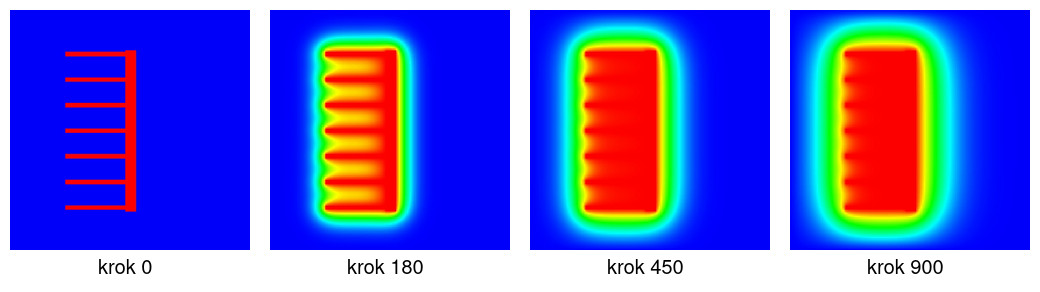
\includegraphics[width=\linewidth]{diffusion_2d.png}
  \caption[Ewolucja pola dyfuzji 2D]{Ewolucja pola temperatury w~dwuwymiarowej
  symulacji dyfuzji, wykonana dwuwymiarowym programem Chapel (dziedzina
  \num{160}$\times$\num{160}). Od~lewej: początkowe, podtrzymywane źródło ciepła
  w~kształcie grzebienia, a~następnie stopniowe wygładzanie ostrych szczegółów
  i~propagacja ciepła w~otoczenie, aż do~ukształtowania się gładkiego gradientu.
  Barwa odwzorowuje temperaturę: błękit oznacza zimno, czerwień gorąco. Ta
  sama zasada obowiązuje w~przypadku trójwymiarowym rozważanym w~pracy.}
  \label{fig:diffusion}
\end{figure}

\subsection{Dyskretyzacja: jawna metoda różnic skończonych}

Do~rozwiązania równania~\eqref{eq:heat3d} zastosowano jawną metodę różnic
skończonych (ang.\ \emph{Finite Difference Method}, FDM) z~jawnym schematem
Eulera w~czasie i~centralnymi różnicami drugiego rzędu w~przestrzeni~\cite{leveque,strikwerda}. Dziedzinę
ciągłą zastępuje się regularną siatką kartezjańską o~\(n_x\times n_y\times n_z\)
węzłach. Krok siatki w~każdym z~kierunków dobrany jest tak, aby węzły skrajne
pokrywały się z~brzegiem sześcianu jednostkowego:
\begin{equation}
  \Delta x = \frac{1}{n_x-1}, \qquad
  \Delta y = \frac{1}{n_y-1}, \qquad
  \Delta z = \frac{1}{n_z-1}.
  \label{eq:spacing}
\end{equation}
Wartość pola w~węźle \((i,j,k)\) w~kroku czasowym \(n\) oznacza się przez
\(u_{i,j,k}^{\,n}\). Do~przybliżenia pierwszej pochodnej czasowej użyto ilorazu
różnicowego przedniego, a~drugich pochodnych przestrzennych standardowych
trzypunktowych ilorazów centralnych, na~przykład dla~kierunku
\(x\):
\begin{equation}
  \frac{\partial^2 u}{\partial x^2}(x_i,y_j,z_k)
  \approx
  \frac{u_{i-1,j,k}^{\,n} - 2\,u_{i,j,k}^{\,n} + u_{i+1,j,k}^{\,n}}{\Delta x^2},
  \label{eq:central}
\end{equation}
i~analogicznie dla~kierunków \(y\) oraz \(z\). Podstawienie tych przybliżeń
do~\eqref{eq:heat3d} i~rozwiązanie względem wartości w~następnym kroku prowadzi
do~jawnej formuły aktualizacji.

Dla~zwięzłości wprowadza się współczynniki wagowe zależne od~osi, łączące
dyfuzyjność, krok czasowy oraz krok siatki:
\begin{equation}
  a_x = \frac{\alpha\,\Delta t}{\Delta x^2}, \qquad
  a_y = \frac{\alpha\,\Delta t}{\Delta y^2}, \qquad
  a_z = \frac{\alpha\,\Delta t}{\Delta z^2}.
  \label{eq:weights}
\end{equation}
Przy tych oznaczeniach reguła aktualizacji przyjmuje zwartą postać
siedmiopunktowego stencila (ang.\ \emph{7-point stencil}):
\begin{align}
  u_{i,j,k}^{\,n+1} =\; & u_{i,j,k}^{\,n}
    + a_x\!\left(u_{i-1,j,k}^{\,n} - 2\,u_{i,j,k}^{\,n} + u_{i+1,j,k}^{\,n}\right) \notag\\
    & + a_y\!\left(u_{i,j-1,k}^{\,n} - 2\,u_{i,j,k}^{\,n} + u_{i,j+1,k}^{\,n}\right) \notag\\
    & + a_z\!\left(u_{i,j,k-1}^{\,n} - 2\,u_{i,j,k}^{\,n} + u_{i,j,k+1}^{\,n}\right).
  \label{eq:update}
\end{align}
Nowa wartość w~każdym węźle zależy wyłącznie od~wartości w~tym węźle oraz
w~jego sześciu bezpośrednich sąsiadach z~poprzedniego kroku czasowego: dwóch
wzdłuż każdej z~trzech osi. Ten wzorzec dostępu do~pamięci, komórka centralna
plus sześć sąsiadów, przedstawiono na~\cref{fig:stencil}. Zależność od~stanu
wyłącznie z~poprzedniego kroku jest cechą schematu jawnego i~czyni każdy krok
czasowy w~pełni równoległym względem węzłów siatki.

\begin{figure}[htbp]
  \centering
  \begin{tikzpicture}[scale=1.0,
      cell/.style={circle,draw,thick,minimum size=7mm,inner sep=0pt},
      center/.style={circle,draw,thick,fill=codekw!18,minimum size=7.5mm,inner sep=0pt},
      nb/.style={circle,draw,thick,fill=codestr!12,minimum size=7mm,inner sep=0pt},
      arr/.style={-{Latex[length=2mm]},thick,gray}]
    % central node
    \node[center] (C) at (0,0) {\small $u_{i,j,k}$};
    % x-neighbours
    \node[nb] (Xm) at (-2.6,0) {\small $u_{i\text{-}1}$};
    \node[nb] (Xp) at ( 2.6,0) {\small $u_{i\text{+}1}$};
    % y-neighbours (vertical)
    \node[nb] (Ym) at (0,-2.2) {\small $u_{j\text{-}1}$};
    \node[nb] (Yp) at (0, 2.2) {\small $u_{j\text{+}1}$};
    % z-neighbours (diagonal, pseudo-3D)
    \node[nb] (Zm) at (-1.5,-1.25) {\small $u_{k\text{-}1}$};
    \node[nb] (Zp) at ( 1.5, 1.25) {\small $u_{k\text{+}1}$};
    % connections
    \foreach \n in {Xm,Xp,Ym,Yp,Zm,Zp} \draw[arr] (\n) -- (C);
    % axis labels
    \node[gray] at (2.6,-0.55) {\footnotesize oś $x$};
    \node[gray] at (0.75,2.2) {\footnotesize oś $y$};
    \node[gray] at (1.9,0.55) {\footnotesize oś $z$};
  \end{tikzpicture}
  \caption[Stencil siedmiopunktowy 3D]{Siedmiopunktowy stencil trójwymiarowy.
  Nowa wartość w~komórce centralnej \(u_{i,j,k}\), zaznaczonej na~niebiesko, jest ważoną
  kombinacją jej wartości bieżącej oraz sześciu bezpośrednich sąsiadów
  zaznaczonych na~czerwono, wzdłuż osi \(x\), \(y\) i~\(z\), zgodnie z~równaniem~\eqref{eq:update}.}
  \label{fig:stencil}
\end{figure}

\subsection{Stabilność numeryczna i warunek CFL}
\label{sec:cfl}

Zaletą schematów jawnych jest prostota i~niski koszt pojedynczego kroku: nie wymagają one rozwiązywania układów równań, w~przeciwieństwie do~schematów
niejawnych. Ceną za~tę prostotę jest jednak warunkowa stabilność: krok czasowy
\(\Delta t\) nie może być dowolnie duży~\cite{leveque,morton-mayers}. Zbyt duży krok powoduje, że błędy
zaokrągleń i~składowe wysokoczęstotliwościowe rozwiązania numerycznego są
wzmacniane w~każdej iteracji zamiast tłumione, co prowadzi do~gwałtownej,
niefizycznej rozbieżności rozwiązania.

Analiza stabilności metodą von~Neumanna~\cite{strikwerda,leveque} dla~schematu
jawnego zastosowanego do~równania dyfuzji w~trzech wymiarach prowadzi do~warunku
Couranta--Friedrichsa--Lewy'ego (CFL). Dla~liniowego schematu o~stałych
współczynnikach współczynnik wzmocnienia pojedynczego modu Fouriera wynosi
\(g = 1 - 4a_x\sin^2(\theta_x/2) - 4a_y\sin^2(\theta_y/2) - 4a_z\sin^2(\theta_z/2)\),
a~żądanie \(\lvert g\rvert\le 1\) dla~najbardziej niekorzystnego modu o~naprzemiennym
znaku między sąsiednimi węzłami redukuje się do~nierówności
\(a_x+a_y+a_z\le\tfrac12\): sumaryczna waga dyfuzyjna nie może przekraczać jednej
drugiej, co wyznacza maksymalny dopuszczalny krok czasowy:
\begin{equation}
  \Delta t_{\max}
  = \frac{1}{2\alpha\!\left(\dfrac{1}{\Delta x^2}
    + \dfrac{1}{\Delta y^2} + \dfrac{1}{\Delta z^2}\right)}.
  \label{eq:cfl}
\end{equation}
Zależność~\eqref{eq:cfl} ma istotne konsekwencje praktyczne: dwukrotne
zagęszczenie siatki wymusza czterokrotne
zmniejszenie kroku czasowego, a~zatem czterokrotny wzrost liczby kroków
potrzebnych do~przebycia tego samego przedziału czasu fizycznego. Wraz
z~ośmiokrotnym wzrostem liczby węzłów siatki daje to bardzo
szybki wzrost całkowitego nakładu obliczeniowego, jedna z~przyczyn, dla~których
symulacje dużych siatek wymagają obliczeń rozproszonych.

W~zaimplementowanym programie krok czasowy dobierany jest automatycznie
na~podstawie warunku~\eqref{eq:cfl}, z~zastosowaniem współczynnika bezpieczeństwa
\num{0.98}:
\begin{equation}
  \Delta t = \num{0.98}\cdot\Delta t_{\max}.
  \label{eq:dt}
\end{equation}
Ten \SI{2}{\percent} margines (ang.\ \emph{safety back-off}) spycha punkt pracy
poniżej granicy stabilności (\(g=\num{-0.96}\) dla~najbardziej niekorzystnego
modu), dzięki czemu schemat pozostaje po~stabilnej stronie nawet przy
uwzględnieniu błędów zaokrągleń arytmetyki zmiennoprzecinkowej i~drobnych efektów
numerycznych, które mogłyby zepchnąć krok dokładnie na~granicy w~obszar
niestabilności. Wybór
wartości bliskiej jedności jest jednocześnie korzystny wydajnościowo:
maksymalizuje postęp w~czasie fizycznym na~jeden krok obliczeniowy, minimalizując
liczbę wymaganych iteracji, a~tym samym liczbę kosztownych wymian danych między
węzłami omawianych w~dalszej części rozdziału.

\section{Zrównoleglenie obliczeń stencilowych}
\label{sec:parallel}

\subsection{Dekompozycja dziedziny i komórki brzegowe}

Obliczenia stencilowe należą do~klasy problemów zrównoleglanych przez podział
danych (ang.\ \emph{data parallelism}). Ponieważ aktualizacja
każdego węzła według~\eqref{eq:update} jest niezależna w~obrębie jednego kroku
czasowego, naturalną strategią jest dekompozycja dziedziny (ang.\ \emph{domain
decomposition}): globalna siatka zostaje podzielona na~rozłączne podobszary,
z~których każdy przypisany jest do~osobnej jednostki obliczeniowej, w~rozważanym
przypadku do~osobnego węzła klastra. Każdy węzeł oblicza aktualizację wyłącznie
dla~przydzielonych mu komórek.

Problem pojawia się na~granicach podobszarów. Aby zaktualizować komórki leżące
tuż przy krawędzi swojego podobszaru, węzeł potrzebuje wartości sąsiadów
znajdujących się już w~podobszarze sąsiedniego węzła. Rozwiązaniem jest
otoczenie każdego lokalnego podobszaru dodatkową warstwą komórek brzegowych
(ang.\ \emph{ghost cells} lub \emph{halo}), które przechowują kopie wartości
z~krawędzi sąsiednich podobszarów. W~terminologii Chapel warstwa ta nosi nazwę
\emph{fluff}; w~zaimplementowanym programie zadeklarowano ją o~grubości jednej
komórki w~każdym kierunku, \texttt{fluff=(1,1,1)}, co odpowiada zasięgowi
siedmiopunktowego stencila. \Cref{fig:domain} przedstawia schematycznie podział
dziedziny na~podobszary wraz z~warstwami brzegowymi.

\begin{figure}[htbp]
  \centering
  \begin{tikzpicture}[scale=0.95,
      core/.style={rectangle,draw=blue!55!black,thick,minimum height=20mm,minimum width=20mm,fill=blue!16},
      halo/.style={rectangle,draw=red!70!black,dashed,thick,minimum height=20mm,minimum width=4mm,fill=red!16},
      lab/.style={font=\footnotesize},
      exch/.style={{Latex[length=2mm]}-{Latex[length=2mm]},thick,codestr}]
    % three locales side by side
    \foreach \i/\x in {0/0, 1/3.2, 2/6.4} {
      \node[core] (L\i) at (\x,0) {locale \i};
    }
    % halo strips between locales (right halo of L_i / left halo of L_{i+1})
    \node[halo] (h0r) at (1.2,0) {};
    \node[halo] (h1l) at (2.0,0) {};
    \node[halo] (h1r) at (4.4,0) {};
    \node[halo] (h2l) at (5.2,0) {};
    % exchange arrows
    \draw[exch] (1.2,1.3) -- (2.0,1.3);
    \draw[exch] (4.4,1.3) -- (5.2,1.3);
    \node[lab,codestr] at (1.6,1.7) {updateFluff()};
    \node[lab,codestr] at (4.8,1.7) {updateFluff()};
    % opisy z liniami odniesienia (rozsunięte, aby się nie nakładały)
    \node[lab] (lc0) at (0,-2.5) {podobszar};
    \draw[thin,gray] (lc0.north) -- (0,-1.05);
    \node[lab] (lc1) at (3.2,-2.6) {\shortstack{obliczenia\\ lokalne}};
    \draw[thin,gray] (lc1.north) -- (3.2,-1.05);
    \node[lab] (lf) at (1.6,-3.6) {warstwa brzegowa (\emph{fluff})};
    \draw[thin,gray] (lf.north) -- (1.2,-1.05);
    % kierunek, wzdłuż którego globalna siatka jest cięta na plastry
    \draw[-{Latex[length=3mm]},thick,gray] (-1.6,-4.5) -- (8.2,-4.5);
    \node[lab,gray] at (3.2,-4.95)
      {kierunek podziału globalnej siatki na~plastry};
  \end{tikzpicture}
  \caption[Dekompozycja dziedziny z~warstwami brzegowymi]{Dekompozycja dziedziny
  w~postaci plastrów (ang.\ \emph{slab decomposition}) na~trzy jednostki
  (\emph{locale}). Globalna siatka jest cięta wzdłuż jednej osi, którą wskazuje strzałka na~dole;
  każdy podobszar, zaznaczony na~niebiesko, otoczony jest warstwą komórek brzegowych
  \emph{fluff}, zaznaczoną na~czerwono linią przerywaną, przechowującą kopie krawędzi
  sąsiadów. Przed~każdym krokiem obliczeń wywołanie \texttt{updateFluff()}
  realizuje wymianę brzegów z~najbliższymi sąsiadami.}
  \label{fig:domain}
\end{figure}

\subsection{Wymiana brzegów jako jedyna komunikacja}

W~każdym kroku czasowym warstwy brzegowe muszą zostać odświeżone, zanim rozpocznie
się faza obliczeń, gdyż przechowywane w~nich wartości pochodzą z~poprzedniego
kroku sąsiedniego węzła. Ta wymiana danych z~najbliższymi sąsiadami
(ang.\ \emph{nearest-neighbour} lub \emph{halo exchange}) jest jedynym rodzajem
komunikacji między węzłami wymaganym przez schemat jawny. W~zaimplementowanym
programie realizuje ją pojedyncze wywołanie metody \texttt{updateFluff()} biblioteki
rozkładów Chapel, wykonywane na~początku każdego kroku, przed~pętlą aktualizującą
wnętrze dziedziny.

Prowadzi to do~wyraźnego rozdziału każdego kroku czasowego na~dwie fazy:
fazę komunikacji, czyli odświeżenie warstw brzegowych, oraz fazę obliczeń, czyli wykonanie
formuły~\eqref{eq:update} dla~wszystkich komórek wnętrza. W~programie fazy te są
oddzielnie mierzone stoperami \texttt{fluffTimer} i~\texttt{computeTimer}, co
pozwala precyzyjnie rozdzielić czas spędzony na~komunikacji od~czasu obliczeń
i~stanowi podstawę analizy skalowalności w~dalszych rozdziałach. Struktura
pojedynczego kroku jest zwięźle widoczna w~procedurze \texttt{stepOnce},
przedstawionej na~\cref{lst:steponce-idea}: najpierw synchronizacja brzegów, potem
równoległa aktualizacja wnętrza.

\begin{lstlisting}[language=Chapel,caption={Pojedynczy krok czasowy: wymiana
brzegów, a~następnie równoległa aktualizacja wnętrza dziedziny.},label={lst:steponce-idea}]
proc stepOnce(ref dst, ref src, ref fluffTimer, ref computeTimer) {
  fluffTimer.start();
  src.updateFluff();               // jedyna komunikacja: wymiana halo
  fluffTimer.stop();
  computeTimer.start();
  forall (i,j,k) in interior do    // faza obliczeń, w pełni równoległa
    dst[i,j,k] = src[i,j,k]
      + ax * (src[i-1,j,k] - 2*src[i,j,k] + src[i+1,j,k])
      + ay * (src[i,j-1,k] - 2*src[i,j,k] + src[i,j+1,k])
      + az * (src[i,j,k-1] - 2*src[i,j,k] + src[i,j,k+1]);
  computeTimer.stop();
}
\end{lstlisting}

\subsection{Intensywność arytmetyczna i ograniczenia wydajności}

Kluczową cechą obliczeń stencilowych, decydującą o~ich zachowaniu wydajnościowym,
jest bardzo niska \emph{intensywność arytmetyczna} (ang.\ \emph{arithmetic
intensity})~\cite{datta-stencil}, iloraz liczby wykonanych operacji zmiennoprzecinkowych do~liczby
bajtów przeniesionych z~pamięci. Aktualizacja jednego węzła według~\eqref{eq:update}
wymaga zaledwie kilkunastu operacji zmiennoprzecinkowych, sześciu odejmowań, trzech
mnożeń przez wagi i~kilku dodawań, a~jednocześnie odczytu siedmiu wartości
i~zapisu jednej, przy \SI{8}{\byte} na~liczbę w~podwójnej precyzji daje to
zaledwie ułamek operacji na~każdy przeniesiony bajt. Co więcej, sąsiednie węzły
współdzielą większość odczytów, lecz nawet przy idealnym wykorzystaniu pamięci
podręcznej stosunek ten pozostaje niski.

Konsekwencją jest to, że wydajność obliczeń stencilowych nie jest ograniczona
przez moc obliczeniową procesora, lecz przez przepustowość transferu danych.
W~ujęciu modelu \emph{roofline}~\cite{roofline} punkt pracy tego typu zadania leży daleko
po~lewej stronie wykresu, w~obszarze ograniczonym nachyloną prostą przepustowości
pamięci, a~nie poziomą półką szczytowej wydajności obliczeniowej. Na~pojedynczym
węźle oznacza to ograniczenie przepustowością pamięci (ang.\ \emph{memory-bandwidth
bound}): dodawanie kolejnych rdzeni obliczeniowych przynosi coraz mniejsze
korzyści, gdy magistrala pamięci ulega nasyceniu. W~obliczeniach rozproszonych,
gdzie warstwy brzegowe muszą przejść przez sieć, zadanie staje się ograniczone
komunikacją (ang.\ \emph{communication bound}): o~całkowitym czasie decyduje
przepustowość i~opóźnienie połączeń sieciowych między węzłami, a~nie szybkość
samych obliczeń.

Zależność ta ma jednak korzystny aspekt związany ze~skalą problemu. Objętość
obliczeń w~podobszarze rośnie proporcjonalnie do~jego objętości, czyli jak
\(N^3\) dla~sześcianu o~boku \(N\), podczas gdy objętość danych brzegowych
podlegających wymianie rośnie proporcjonalnie do~pola powierzchni granic,
czyli jak \(N^2\). Stosunek nakładu obliczeń do~nakładu komunikacji jest zatem
rzędu \(N^3/N^2 = N\) i~rośnie liniowo z~rozmiarem krawędzi siatki. Innymi słowy,
większe sześciany mają korzystniejszy stosunek obliczeń do~komunikacji: koszt
komunikacji zostaje zamortyzowany większą liczbą obliczeń przypadających
na~każdy przesłany bajt. Obserwacja ta ma bezpośrednie przełożenie na~strategię
efektywnego skalowania i~zostanie potwierdzona empirycznie w~rozdziale
z~wynikami.

\subsection{Miary skalowalności}

Do~ilościowej oceny efektywności zrównoleglenia stosuje się standardowy aparat
pojęciowy. \emph{Przyspieszenie} (ang.\ \emph{speedup}) przy użyciu \(p\)
jednostek obliczeniowych definiuje się jako stosunek czasu wykonania sekwencyjnego
do~czasu wykonania równoległego:
\begin{equation}
  S(p) = \frac{T(1)}{T(p)},
  \label{eq:speedup}
\end{equation}
a~\emph{efektywność równoległą} (ang.\ \emph{parallel efficiency}) jako
przyspieszenie znormalizowane liczbą jednostek:
\begin{equation}
  E(p) = \frac{S(p)}{p} = \frac{T(1)}{p\,T(p)}.
  \label{eq:efficiency}
\end{equation}
Idealne, liniowe przyspieszenie odpowiada \(S(p)=p\) oraz \(E(p)=1\); w~praktyce
narzuty komunikacji, synchronizacji i~nierównomiernego obciążenia sprawiają,
że \(E(p)<1\), przy czym efektywność zwykle maleje ze~wzrostem \(p\).

Rozróżnia się dwa reżimy badania skalowalności. \emph{Skalowanie mocne}
(ang.\ \emph{strong scaling}) polega na~ustaleniu całkowitego rozmiaru problemu
i~zwiększaniu liczby jednostek obliczeniowych; celem jest skrócenie czasu
rozwiązania. W~tym reżimie udział pracy przypadającej na~jednostkę maleje,
przez co narzuty komunikacyjne stają się względnie coraz istotniejsze, a~granicę
osiągalnego przyspieszenia opisuje prawo Amdahla. \emph{Skalowanie słabe}
(ang.\ \emph{weak scaling}) polega na~ustaleniu rozmiaru problemu przypadającego
na~jedną jednostkę i~proporcjonalnym zwiększaniu zarówno liczby jednostek, jak
i~całkowitego rozmiaru problemu; celem jest rozwiązywanie coraz większych
zadań w~stałym czasie.

Fundamentalne ograniczenie skalowania mocnego formułuje \emph{prawo Amdahla}~\cite{amdahl}.
Jeśli \(f\) oznacza sekwencyjną część obliczeń, której z~natury nie da się zrównoleglić, to maksymalne osiągalne przyspieszenie przy \(p\) jednostkach
wynosi
\begin{equation}
  S(p) \le \frac{1}{f + \dfrac{1-f}{p}},
  \qquad
  \lim_{p\to\infty} S(p) = \frac{1}{f}.
  \label{eq:amdahl}
\end{equation}
Nawet niewielki udział części sekwencyjnej narzuca zatem twardą górną granicę
przyspieszenia, niezależnie od~liczby dostępnych jednostek. W~kontekście
rozważanego programu rolę nieusuwalnego narzutu pełni głównie komunikacja, wymiana warstw brzegowych, oraz synchronizacja między krokami,
co, w~połączeniu z~ograniczeniem przepustowością pamięci i~sieci omówionym
wcześniej, wyznacza realistyczne granice skalowalności analizowane w~dalszej
części pracy.

\section{Chapel, PGAS i GASNet}
\label{sec:chapel}

\subsection{Język Chapel i model PGAS}

Implementację programu oparto na~języku Chapel, języku programowania
równoległego rozwijanym z~myślą o~produktywności programisty przy zachowaniu
wysokiej wydajności na~systemach wieloprocesorowych i~rozproszonych~\cite{chapel-overview,chapel-book}. Chapel
realizuje model \emph{PGAS} (ang.\ \emph{Partitioned Global Address Space},
partycjonowana globalna przestrzeń adresowa)~\cite{pgas,upc}. Idea PGAS polega na~tym, że pamięć
wszystkich węzłów tworzy jedną logicznie wspólną przestrzeń adresową, która
jest jednak podzielona na~partycje o~jawnie określonym powinowactwie do~węzłów.
Programista operuje na~danych za~pomocą jednolitej, globalnej perspektywy
(ang.\ \emph{global-view}), tak jakby były one lokalne, natomiast środowisko
uruchomieniowe automatycznie tłumaczy dostępy do~danych zdalnych na~operacje
komunikacji sieciowej. Model ten łączy wygodę programowania w~pamięci wspólnej
z~wydajnościową świadomością rozmieszczenia danych, charakterystyczną dla~modelu
przekazywania komunikatów.

Centralnym pojęciem w~Chapel jest \emph{locale}, abstrakcja jednostki
systemu dysponującej własną pamięcią oraz zdolnością do~wykonywania obliczeń.
W~konfiguracji wielowęzłowej stosowanej w~niniejszej pracy każdemu węzłowi
fizycznemu klastra odpowiada dokładnie jeden locale, w~odwzorowaniu
\emph{jeden-do-jednego}. Wbudowana tablica \texttt{Locales} udostępnia wszystkie
dostępne jednostki, a~ich liczbę podaje stała \texttt{numLocales}. Dostęp
do~danych i~przenoszenie obliczeń pomiędzy jednostkami wyraża się wprost,
za~pomocą konstrukcji \texttt{on}.

\subsection{Iteratory równoległe i tablice globalne}

Chapel oferuje dwa uzupełniające się rodzaje równoległości. Równoległość danych
wyraża pętla \texttt{forall}, która zleca wykonanie ciała iteracji dla~wszystkich
elementów dziedziny współbieżnie, pozostawiając środowisku uruchomieniowemu
podział pracy na~zadania i~przypisanie ich do~wątków. W~programie to właśnie
pętla \texttt{forall} nad~dziedziną wnętrza (\cref{lst:steponce-idea}) realizuje fazę
obliczeń stencila. Gdy pętla iteruje po~dziedzinie rozproszonej, jej iteracje
wykonują się na~tych węzłach, do~których przypisane są odpowiednie elementy,
co zapewnia lokalność obliczeń bez~jawnego zarządzania nią przez programistę.

Równoległość zadaniową między węzłami wyraża konstrukcja
\texttt{coforall \ldots on loc}, która tworzy osobne zadanie dla~każdego locale
i~umieszcza jego wykonanie na~odpowiednim węźle. W~programie wzorzec ten
wykorzystywany jest między innymi do~równoległego zapisu klatek wynikowych, każdy węzeł niezależnie zapisuje swój lokalny podobszar. \Cref{lst:coforall}
ilustruje ten idiom.

\begin{lstlisting}[language=Chapel,caption={Równoległość zadaniowa między węzłami:
każdy locale wykonuje operację na~swoim lokalnym podobszarze danych.},label={lst:coforall}]
coforall loc in Locales do on loc {
  const ld = field.localSubdomain();   // lokalny fragment tablicy globalnej
  var block: [ld] real = field[ld];    // kopia danych bez komunikacji zdalnej
  // ... zapis / obliczenia lokalne na fragmencie ...
}
\end{lstlisting}

Tablice w~Chapel definiowane są nad~\emph{dziedzinami} (ang.\ \emph{domain}), obiektami opisującymi zbiór indeksów. Aby tablica została rozproszona pomiędzy
węzły, jej dziedzinę wyposaża się w~\emph{odwzorowanie dziedziny}
(ang.\ \emph{domain map}, dystrybucję). Najprostszą dystrybucją jest \texttt{Block},
dzieląca zakres indeksów na~w~przybliżeniu równe, przylegające bloki i~przypisująca
je kolejnym węzłom. Na~potrzeby obliczeń stencilowych Chapel udostępnia
wyspecjalizowaną dystrybucję \texttt{Stencil} z~modułu \texttt{StencilDist}, która
poza~podziałem danych utrzymuje wokół każdego lokalnego bloku warstwę komórek
brzegowych \emph{fluff}, przechowującą buforowane kopie krawędzi sąsiadów.
Warstwę tę odświeża się jawnym wywołaniem \texttt{updateFluff()}, co realizuje
opisaną wcześniej wymianę \emph{halo}~\cite{stencildist}. W~programie dziedzinę tworzy się wywołaniem
\texttt{stencilDist.\allowbreak createDomain(\ldots,\allowbreak{} fluff=(1,1,1))},
zapewniając brzeg
o~grubości jednej komórki, dokładnie odpowiadający zasięgowi
stencila~\eqref{eq:update}.

\subsection{Warstwa zadań qthreads oraz warstwa komunikacji GASNet}

Wykonanie zadań w~obrębie pojedynczego locale spoczywa na~warstwie szeregowania
zadań. W~zastosowanej konfiguracji jest to biblioteka \emph{qthreads}
(\texttt{CHPL\_TASKS=qthreads}), lekki system wątków użytkownika efektywnie
obsługujący dużą liczbę drobnoziarnistych zadań generowanych przez pętle
\texttt{forall}~\cite{qthreads}. Liczbę wątków sprzętowych dostępnych na~danym węźle udostępnia
własność \texttt{here.maxTaskPar}; wyznacza ona stopień równoległości fazy
obliczeń w~obrębie węzła i~jest raportowana przez program przy starcie.

Za~komunikację między węzłami odpowiada z~kolei warstwa \emph{GASNet}, przenośna biblioteka uruchomieniowa dostarczająca prymitywów komunikacji
jednostronnej (ang.\ \emph{one-sided}) oraz komunikatów aktywnych, na~których
Chapel opiera realizację dostępów do~pamięci zdalnej i~operacji \texttt{on}~\cite{gasnet,gasnet-spec}.
Uaktywnia się ją ustawieniem \texttt{CHPL\_COMM=gasnet}. W~zastosowanej
konfiguracji przyjęto tryb segmentu
\texttt{CHPL\_\allowbreak GASNET\_\allowbreak SEGMENT\allowbreak =everything},
w~którym cała pamięć procesu jest udostępniana dla~komunikacji zdalnej, co
upraszcza rozmieszczanie tablic rozproszonych. Warstwową strukturę całego
stosu, od~kodu aplikacji, przez model globalnej tablicy PGAS, aż po~sprzęt
sieciowy, przedstawia \cref{fig:layers}.

\begin{figure}[htbp]
  \centering
  \begin{tikzpicture}[
      layer/.style={rectangle,draw,thick,minimum width=82mm,minimum height=9mm,
                    align=center,font=\small},
      lab/.style={font=\footnotesize\itshape,gray}]
    \node[layer,fill=codekw!16] (app) {Aplikacja: program 3D (stencil, \texttt{forall}, \texttt{updateFluff})};
    \node[layer,fill=codekw!12,below=2mm of app] (chpl) {Chapel: tablice globalne PGAS, \texttt{locale}, dystrybucja \texttt{Stencil}};
    \node[layer,fill=codestr!10,below=2mm of chpl] (rt) {Warstwa uruchomieniowa: zadania \texttt{qthreads} \;$\;\vert\;$\; komunikacja \texttt{GASNet}};
    \node[layer,fill=codestr!14,below=2mm of rt] (cond) {Konduit GASNet: \texttt{udp} (AMUDP) \; / \; \texttt{mpi} (nad~MPICH/TCP)};
    \node[layer,fill=black!8,below=2mm of cond] (net) {Sieć węzłów klastra (Ethernet / TCP-IP)};
    \draw[{Latex[length=2mm]}-{Latex[length=2mm]},thick] (app) -- (chpl);
    \draw[{Latex[length=2mm]}-{Latex[length=2mm]},thick] (chpl) -- (rt);
    \draw[{Latex[length=2mm]}-{Latex[length=2mm]},thick] (rt) -- (cond);
    \draw[{Latex[length=2mm]}-{Latex[length=2mm]},thick] (cond) -- (net);
  \end{tikzpicture}
  \caption[Warstwy stosu Chapel/PGAS/GASNet]{Warstwowa architektura wykonania.
  Kod aplikacji operuje na~globalnych tablicach PGAS języka Chapel; ich dostępy
  zdalne i~wymiana warstw brzegowych są realizowane przez warstwę uruchomieniową,
  w~której zadania \texttt{qthreads} wykonują się lokalnie, a~komunikacja \texttt{GASNet}
  zachodzi między~węzłami; warstwa ta korzysta z~kolei z~wybranego konduitu
  odwzorowującego operacje na~fizyczną sieć klastra.}
  \label{fig:layers}
\end{figure}

\subsection{Konduity GASNet}

GASNet abstrahuje sprzęt sieciowy poprzez wymienne \emph{konduity}
(ang.\ \emph{conduits}), moduły implementujące prymitywy komunikacji
na~konkretnej technologii transportu. W~ramach niniejszej pracy porównywano dwa
konduity dostępne na~klastrze zbudowanym z~węzłów połączonych zwykłą siecią
Ethernet. Konduit \texttt{udp}, oparty na~warstwie AMUDP, realizuje komunikaty
aktywne bezpośrednio nad~datagramami UDP i~jest uruchamiany za~pomocą programu
rozruchowego \texttt{amudprun}. Jego zaletą jest prostota konfiguracji, wadą zaś
podatność na~przeciążenie przy intensywnej, drobnoziarnistej wymianie danych.
Konduit \texttt{mpi} przenosi komunikację GASNet na~istniejącą implementację
MPI, w~zastosowanej konfiguracji opartej na~MPICH nad~TCP, i~jest uruchamiany
programem \texttt{gasnetrun\_mpi}; zapewnia on stabilniejszy i~wydajniejszy
transport dla~podtrzymywanych, regularnych wzorców komunikacji, jakie generuje
cykliczna wymiana warstw brzegowych w~opisywanym programie.

Wybór konduitu okazuje się mieć istotny wpływ na~zachowanie rozproszonej
symulacji, ponieważ, jak wykazano w~\cref{sec:parallel}, w~reżimie
wielowęzłowym zadanie jest ograniczone komunikacją, a~jedyną komunikacją
per~krok jest wymiana \emph{halo} realizowana przez \texttt{updateFluff()}.
To właśnie właściwości warstwy komunikacyjnej, jej przepustowość, opóźnienie
oraz odporność na~przeciążenie, decydują w~praktyce o~osiąganej skalowalności,
co czyni dobór konduitu jednym z~centralnych zagadnień badawczych analizowanych
w~dalszej części pracy.

\chapter{Klaster i implementacja}
\label{ch:implementacja}

\section{Architektura klastra i środowisko}
\label{sec:klaster}

\subsection{Sprzęt i topologia}

Docelowym środowiskiem uruchomieniowym jest rzeczywisty klaster \emph{Pionier} w~pracowni komputerowej Wydziału Matematyki i~Informatyki UMK, złożony z~dziewięciu jednorodnych węzłów fizycznych (\emph{Pionier-lab8-1}\,\dots\,\emph{Pionier-lab8-9}) połączonych przełącznikiem Ethernet o~przepustowości \SI{1}{Gb\per\second}. Wszystkie węzły są identyczne: każdy wyposażony jest w~procesor Intel Core i7-12700K (\num{12} rdzeni, \num{20} wątków sprzętowych), \SI{32}{GiB} pamięci RAM DDR4-3200 oraz kartę sieciową Intel I219-V (sterownik \texttt{e1000e}, \SI{1}{Gb\per\second}) i~pracuje pod systemem Ubuntu (jądro \texttt{6.8.0-111-generic}). Węzły mają adresy z~podsieci \texttt{192.168.128.0/24}, a~dostęp do nich odbywa się bezpośrednim poleceniem \texttt{ssh <ip>}. Jednorodność środowiska, czyli ta sama architektura procesora, dystrybucja i~wersja bibliotek na każdym węźle, upraszcza dystrybucję binariów: obraz zbudowany na jednym węźle działa bez zmian na pozostałych. W~eksperymentach skalowania każdemu węzłowi fizycznemu odpowiadał jeden lokal (\emph{locale}), co pozwoliło zbadać skalowanie w~funkcji liczby węzłów aż do dziewięciu.

Topologię środowiska przedstawiono na \cref{fig:topologia}. Warto zauważyć, że wszystkie węzły dzielą jedno łącze o~przepustowości \SI{1}{Gb\per\second}. To łącze jest wąskim gardłem komunikacji rozproszonej, bo każda wymiana komórek brzegowych między sąsiednimi fragmentami dziedziny przechodzi przez ten sam przełącznik.

\begin{figure}[H]
  \centering
  \begin{tikzpicture}[
      node distance=8mm,
      box/.style={draw, rounded corners, minimum width=24mm, minimum height=15mm, align=center, thick},
      switch/.style={draw, fill=black!8, minimum width=96mm, minimum height=10mm, align=center, thick},
      link/.style={very thick},
    ]
    \node[box] (n1) {\textbf{lab8-1}\\[1pt] i7-12700K\\ \num{20} wątków, \SI{32}{GiB}};
    \node[box, right=8mm of n1] (n2) {\textbf{lab8-2}\\[1pt] i7-12700K\\ \num{20} wątków, \SI{32}{GiB}};
    \node[right=8mm of n2] (dots) {\Large$\cdots$};
    \node[box, right=8mm of dots] (n9) {\textbf{lab8-9}\\[1pt] i7-12700K\\ \num{20} wątków, \SI{32}{GiB}};
    \node[switch, below=16mm of $(n1)!0.5!(n9)$] (sw) {przełącznik Ethernet \SI{1}{Gb\per\second}};
    \foreach \n in {n1,n2,n9} \draw[link] (\n.south) -- (\n.south |- sw.north);
    \draw[link, dashed] (dots) -- (dots |- sw.north);
  \end{tikzpicture}
  \caption[Topologia klastra Pionier]{Topologia jednorodnego, dziewięciowęzłowego klastra Pionier. Wszystkie identyczne węzły (\emph{Pionier-lab8-1}\,\dots\,\emph{Pionier-lab8-9}) połączone są jednym przełącznikiem \SI{1}{Gb\per\second}, który stanowi współdzielone i~zarazem najwęższe łącze komunikacji rozproszonej. Środowisko budowane jest raz na dowolnym węźle, a~binaria rozprowadzane na pozostałe.}
  \label{fig:topologia}
\end{figure}

\subsection{Konfiguracja kompilatora Chapel}

Kompilator Chapel w~wersji \num{2.9.0} zbudowano ze źródeł na jednym węźle~\cite{chapel-docs}. Kluczowe parametry środowiska są ,,zapieczone'' w~pliku \texttt{chplconfig}, który skrypt \path{distribute-chapel.sh} zapisuje jeszcze przed wywołaniem \texttt{make}. Dzięki temu każdy węzeł otrzymuje binaria zbudowane z~identyczną konfiguracją. Zawartość istotnej części pliku konfiguracyjnego przedstawia \cref{lst:chplconfig}.

\begin{lstlisting}[style=bash, caption={Fragment pliku \texttt{chplconfig} generowanego przed budową kompilatora.}, label={lst:chplconfig}]
CHPL_COMM=gasnet
CHPL_COMM_SUBSTRATE=$CONDUIT      # udp (domyslnie) albo mpi
CHPL_LLVM=none                    # backend C, nie LLVM
CHPL_TARGET_CPU=$TARGET_CPU       # native
\end{lstlisting}

Warstwą komunikacyjną jest GASNet (\texttt{CHPL\_COMM=gasnet}), co umożliwia pracę wielolokalową. Kompilacja odbywa się z~użyciem backendu C (\texttt{CHPL\_LLVM=none}) zamiast LLVM. Ustawienie \texttt{CHPL\_TARGET\_CPU=native} pozwala na generowanie kodu wykorzystującego pełen zestaw instrukcji procesora hosta; jest to bezpieczne wyłącznie dlatego, że produkcyjny klaster jest jednorodny pod względem architektury procesorów. Z~konfiguracji wynikają dalsze, domyślne wartości środowiska: \texttt{CHPL\_TASKS=qthreads}, \texttt{CHPL\_GASNET\_SEGMENT=everything}, \texttt{CHPL\_LOCALE\_MODEL=flat} oraz \texttt{CHPL\_TARGET\_MEM=jemalloc}. Launcher zależy od wybranego kanału komunikacyjnego i~przyjmuje wartość \texttt{amudprun} dla kanału udp albo \texttt{gasnetrun\_mpi} dla kanału mpi.

\subsection{Dwa kanały komunikacyjne GASNet}

Warstwę GASNet można zbudować na dwóch różnych kanałach transportowych (\emph{conduit}), wybieranych parametrem \texttt{-{}-conduit}~\cite{gasnet-spec}. Kanał \textbf{udp} realizuje protokół AMUDP nad UDP; nie ma dodatkowych zależności i~jest szybki w~czystej sieci lokalnej, jednak przy dużej skali załamuje się z~błędem \texttt{ECONGESTION} w~sytuacji wielu-do-jednego (\emph{incast}) oraz przy utracie pakietów~\cite{incast}. Kanał \textbf{mpi} realizuje GASNet mpi-conduit nad biblioteką MPICH pracującą w~trybie \texttt{ch3:sock}, czyli zwykłym TCP; mechanizm kontroli przepływu TCP przetrwa utratę pakietów i~zjawisko incast~\cite{mpich,mpi-standard}. Ze względu na to, że wybór kanału zapisany jest w~pliku \texttt{chplconfig}, dla każdego kanału utrzymywane jest osobne, w~pełni skompilowane drzewo Chapel (ścieżki \path{.../chapel} oraz \path{.../chapel-mpi}).

Biblioteka MPICH w~wersji \num{4.2.3} została zbudowana ze źródeł skryptem \path{build-mpi.sh} do bezuprawnieniowego prefiksu, z~linią konfiguracji przedstawioną w~\cref{lst:mpich}. Budowa ze źródeł zapewnia na każdym węźle \emph{identyczną} wersję i~konfigurację MPI, w~szczególności urządzenie \texttt{ch3:sock}, czyli zwykły TCP, którego mechanizm kontroli przepływu przetrwa incast, czego nie gwarantują pakiety dystrybucyjne, dostarczające zwykle OpenMPI w~domyślnej konfiguracji. Jedno drzewo zbudowane raz jest kopiowane pod tę samą bezwzględną ścieżkę na każdym węźle, co gwarantuje zgodność ABI.

\begin{lstlisting}[style=bash, caption={Linia konfiguracji budowy MPICH ze źródeł.}, label={lst:mpich}]
./configure --prefix=$PREFIX --disable-fortran \
            --with-device=ch3:sock --disable-static
\end{lstlisting}

\subsection{Uruchamianie i samoopisujące się logi}

Dla każdej binarki skrypt \path{compile-and-distribute.sh} (funkcja \texttt{gen\_run\_script}) generuje osobny skrypt uruchomieniowy. Ustawia on zmienne \texttt{CHPL\_HOME} oraz \texttt{PATH}, domyślnie przyjmuje liczbę wątków na lokal równą \texttt{\$(nproc)}, a~przebieg rejestruje do logu o~nazwie zawierającej znacznik czasu (\path{logs/<bin>-YYYYmmdd-HHMMSS.log}). Zasadniczy fragment logiki uruchomieniowej pokazano w~\cref{lst:run}.

\begin{lstlisting}[style=bash, caption={Blok uruchomieniowo-rejestrujący ze skryptu wrappera.}, label={lst:run}]
set -o pipefail
{
  echo "[cfg] threadsPerLocale(requested)=$CHPL_RT_NUM_THREADS_PER_LOCALE numLocales=${NUM_LOCALES}"
  ./${bin} -nl ${NUM_LOCALES} "$@" 2>&1
} | tee "$LOG"
\end{lstlisting}

Log jest samoopisujący dzięki dwóm liniom \texttt{[cfg]}. Pierwsza, pochodząca ze skryptu, ma postać \texttt{[cfg] threadsPerLocale(requested)=N numLocales=M} i~podaje wartości \emph{żądane}. Druga, pochodząca z~programu, ma postać \texttt{[cfg] locale <id> maxTaskPar=<n>} i~podaje \emph{efektywną} liczbę wątków na lokal po ograniczeniu jej przez qthreads do możliwości sprzętu~\cite{qthreads}. Rozróżnienie to jest istotne przy analizie wydajności, ponieważ w~przypadku nadsubskrypcji (\emph{oversubscription}) liczba żądana może przewyższać liczbę faktycznie dostępnych rdzeni. Konfiguracja launchera zależy od kanału: dla mpi ustawiane jest \texttt{MPIRUN\_CMD="mpirun -n \%N -hosts <hosts> <install>/mpi-iface-wrap.sh \%C"}, natomiast dla udp, zmienne \texttt{GASNET\_SSH\_SERVERS} oraz \texttt{GASNET\_MASTERIP}.

Do celowego wywoływania obciążenia sieci służy harness \path{run-nl.sh}. Przeplata on listę serwerów SSH tak, że kolejne lokale trafiają na różne węzły fizyczne, przez co sąsiadujące fragmenty dziedziny w~rozkładzie \texttt{StencilDist} znajdują się na różnych węzłach. W~konsekwencji \emph{każda} operacja pobrania halo przekracza wspólne łącze \SI{1}{Gb\per\second}, tworząc ruch wielu-do-jednego (incast), co uwidacznia błąd \texttt{ECONGESTION} kanału udp.

Ostatnim elementem środowiska jest skrypt \path{mpi-iface-wrap.sh} odpowiedzialny za przypięcie interfejsu sieciowego per ranga na węzłach wielosieciowych. Wybiera on lokalny adres IPv4 z~właściwej podsieci klastra (\texttt{192.168.128.0/24}), pomijając interfejsy wirtualne, czyli mostki \texttt{docker0} i~\texttt{virbr0}, podsieci \texttt{172.16/12} oraz adresy libvirt \texttt{192.168.122.*}, eksportuje \texttt{MPICH\_INTERFACE\_HOSTNAME}, po czym uruchamia program. Bez tego kroku transport \texttt{ch3:sock} może rozgłosić nieroutowalny adres interfejsu, a~wywołanie \texttt{MPI\_Init} kończy się błędem ,,No route to host''.

\subsection{Procedura wdrożenia krok po kroku}
\label{sec:depl:procedura}

Elementy opisane w~poprzednich podrozdziałach tworzą procedurę wdrożenia, od zbudowania środowiska aż po uruchomienie przebiegu. Choć węzły są jednorodne, procedura ta wykracza poza zwykłą kompilację lokalną, ponieważ kolejność kroków oraz miejsce ich wykonania są istotne dla poprawności i~wymagają spójnych ścieżek oraz identycznych drzew Chapel i~MPICH na wszystkich węzłach. Całość podzielono na cztery etapy.

W~\emph{pierwszym etapie} na dowolnie wybranym węźle budowane jest środowisko wykonawcze: kompilator Chapel w~wersji \num{2.9.0} (skryptem \path{distribute-chapel.sh}) oraz biblioteka MPICH w~wersji \num{4.2.3} w~trybie \texttt{ch3:sock} (skryptem \path{build-mpi.sh}). Ponieważ klaster jest jednorodny, wybór węzła budującego jest dowolny, binaria zbudowane na jednym węźle działają na wszystkich pozostałych.

W~\emph{drugim etapie} skompilowane drzewo Chapel jest pakowane do archiwum i~rozsyłane pod \emph{identyczną} ścieżkę bezwzględną na każdym węźle (\cref{lst:depl:distribute}). Identyczność tej ścieżki jest drugim niezmiennikiem całej procedury: warstwa uruchomieniowa Chapel jest kompilowana ze ścieżką \texttt{rpath} wskazującą wprost do drzewa \texttt{CHPL\_HOME}, więc jakakolwiek rozbieżność lokalizacji uniemożliwia dynamiczne odnalezienie bibliotek współdzielonych. Analogicznie, jedno drzewo MPICH zbudowane raz jest strumieniowane pod tę samą ścieżkę na wszystkich węzłach, co gwarantuje zgodność ABI wymaganą przez mpi-conduit.

\begin{lstlisting}[style=bash, caption={Spakowanie i~rozesłanie zbudowanego drzewa pod identyczną ścieżkę.}, label={lst:depl:distribute}]
tar czf chapel-2.9.0-built.tar.gz -C "$CHPL_HOME/.." chapel-2.9.0
for h in $HOSTS; do
  scp chapel-2.9.0-built.tar.gz "$h:$DEST/"
  ssh "$h" "tar xzf $DEST/chapel-2.9.0-built.tar.gz -C $DEST"
done
\end{lstlisting}

W~\emph{trzecim etapie} kompilowane są binaria samego programu i~rozprowadzane na węzły skryptem \path{compile-and-distribute.sh}. Dla każdej binarki kopiowane są \emph{zarówno} plik launchera \texttt{<bin>}, jak i~właściwy obraz wykonywalny \texttt{<bin>\_real}; oba są niezbędne na każdym węźle do uruchomienia wielolokalowego. Skrypt generuje przy tym dedykowany launcher (por.\ \cref{lst:run}), który ustawia \texttt{CHPL\_HOME} i~\texttt{PATH} zgodnie z~rozesłanym drzewem.

W~\emph{czwartym etapie} przebieg uruchamiany jest przez wygenerowany launcher, który wywołuje właściwy program startowy GASNet (\texttt{gasnetrun\_mpi} dla kanału mpi albo \texttt{amudprun} dla kanału udp) i~rozdziela lokale na węzły. Dwa niezmienniki z poprzednich etapów, \emph{identyczna ścieżka \texttt{CHPL\_HOME}} (rpath) oraz \emph{identyczne drzewa Chapel i~MPICH} pod tą samą ścieżką na wszystkich węzłach, są warunkami koniecznymi powodzenia tego etapu. Naruszenie któregokolwiek objawia się dopiero przy ładowaniu bibliotek lub starcie procesów zdalnych, czyli już po udanej kompilacji.

\section{Struktura programu i krok obliczeniowy}
\label{sec:solver}

\subsection{Dziedzina rozproszona z otoczką}

Podstawą implementacji jest trójwymiarowa dziedzina rozproszona między lokale za pomocą rozkładu \texttt{StencilDist}~\cite{stencildist}. Rozkład ten różni się od zwykłego rozkładu blokowego tym, że wokół bloku należącego do każdego lokala rezerwuje dodatkową warstwę komórek, tak zwaną otoczkę (\emph{fluff}), przechowującą kopie komórek brzegowych sąsiadów. Szerokość otoczki dobrano do stosowanego siedmiopunktowego stencila, wynosi ona jedną komórkę w~każdym kierunku. Definicję dziedziny oraz jej wnętrza przedstawia \cref{lst:domain}.

\begin{lstlisting}[language=Chapel, caption={Definicja dziedziny rozproszonej z jednokomórkową otoczką oraz jej wnętrza.}, label={lst:domain}]
const domain3D = stencilDist.createDomain({0..<nx,0..<ny,0..<nz},
                                          fluff=(1,1,1));
const interior = domain3D.expand(-1);
\end{lstlisting}

Wnętrze \texttt{interior} powstaje przez zmniejszenie dziedziny o~jedną komórkę w~każdym kierunku (\texttt{expand(-1)}); obejmuje ono wyłącznie te komórki, dla których siedmiopunktowy stencil ma komplet sąsiadów wewnątrz dziedziny globalnej. Komórki brzegowe dziedziny nie są aktualizowane i~zachowują wartości początkowe, pełniąc rolę warunków brzegowych typu Dirichleta.

\subsection{Pojedynczy krok obliczeniowy}

Pojedynczy krok czasowy realizuje procedura \texttt{stepOnce}, przedstawiona w~\cref{lst:steponce}. Składa się ona z~dwóch wyraźnie rozdzielonych i~osobno mierzonych faz: wymiany halo oraz właściwego obliczenia stencila. Najpierw wywoływana jest metoda \texttt{src.updateFluff()}, która wykonuje wymianę halo, następnie równoległa pętla \texttt{forall} po wnętrzu dziedziny aktualizuje pole zgodnie ze schematem różnic skończonych.

\begin{lstlisting}[language=Chapel, caption={Procedura pojedynczego kroku: wymiana halo, a następnie obliczenie stencila.}, label={lst:steponce}]
proc stepOnce(ref dst, ref src, ref fluffTimer, ref computeTimer) {
  fluffTimer.start(); src.updateFluff(); fluffTimer.stop();
  computeTimer.start();
  forall (i,j,k) in interior do
    dst[i,j,k] = src[i,j,k]
               + ax*(src[i-1,j,k]-2*src[i,j,k]+src[i+1,j,k])
               + ay*(src[i,j-1,k]-2*src[i,j,k]+src[i,j+1,k])
               + az*(src[i,j,k-1]-2*src[i,j,k]+src[i,j,k+1]);
  computeTimer.stop();
}
\end{lstlisting}

Metoda \texttt{updateFluff()} kopiuje komórki brzegowe każdego lokala do otoczek sąsiadów, przesyłając dane poprzez GASNet; jest to \emph{jedyna} komunikacja odbywająca się w~ramach kroku. Na więcej niż jednym lokalu wywołanie to jest \emph{obowiązkowe} dla poprawności: pominięcie go powoduje odczyt nieaktualnych lub niezainicjowanych komórek otoczki, przez co obliczenie przebiega szybciej, lecz daje wynik \emph{cicho błędny}. Dlatego wymiana halo jest jednocześnie gwarancją poprawności i głównym wąskim gardłem obliczeń rozproszonych, bo przy każdym kroku obciąża wspólne łącze \SI{1}{Gb\per\second}. Przebieg pojedynczego kroku wraz z~fazą zapisu ilustruje \cref{fig:pipeline}.

\begin{figure}[H]
  \centering
  \begin{tikzpicture}[
      phase/.style={draw, rounded corners, minimum height=12mm, align=center, thick},
      comm/.style={phase, fill=black!12},
      comp/.style={phase, fill=black!4},
      io/.style={phase, fill=black!8},
      arr/.style={-{Latex}, thick},
    ]
    \node[comm, minimum width=34mm] (fluff) {\texttt{updateFluff()}\\ wymiana halo\\ \scriptsize (GASNet, sieć)};
    \node[comp, minimum width=34mm, right=8mm of fluff] (comp) {\texttt{forall interior}\\ obliczenie stencila\\ \scriptsize (qthreads, lokalnie)};
    \node[io, minimum width=34mm, right=8mm of comp] (save) {\texttt{dumpLocal()}\\ zapis fragmentu\\ \scriptsize (dysk lokalny, opcj.)};
    \draw[arr] (fluff) -- (comp);
    \draw[arr] (comp) -- (save);
    \node[below=2mm of fluff, font=\scriptsize]{\texttt{fluffTimer}};
    \node[below=2mm of comp, font=\scriptsize]{\texttt{computeTimer}};
    \node[below=2mm of save, font=\scriptsize]{\texttt{save=}};
    % pętla powrotna poprowadzona po zewnętrznych bokach i pod podpisami stoperów
    \draw[arr] (save.east) -- ++(7mm,0) -- ++(0,-16mm)
      -- node[below, font=\scriptsize]{kolejny krok} ($(fluff.west)+(-7mm,-16mm)$)
      -- ($(fluff.west)+(-7mm,0)$) -- (fluff.west);
  \end{tikzpicture}
  \caption[Potok pojedynczego kroku programu]{Potok pojedynczego kroku czasowego programu. Faza komunikacyjna (\texttt{updateFluff}) poprzedza lokalne obliczenie stencila, po którym następuje opcjonalny zapis fragmentu na dysk lokalny. Każda faza mierzona jest osobnym stoperem.}
  \label{fig:pipeline}
\end{figure}

\subsection{Pomiar czasu i rejestrowanie}

Program rozdziela pomiar czasu na wyraźnie zdefiniowane obszary. Stoper \texttt{initTimer} obejmuje fazę przygotowania (alokacja tablic, inicjalizacja gorącej warstwy oraz obliczenie kroku czasowego \texttt{dt} i~współczynników), której wynik raportowany jest jako \emph{Initialization time}. Stoper \texttt{computeTimer} obejmuje całą pętlę czasową i~raportowany jest jako \emph{Execution time} (w~wariancie z~zamianą buforów: \emph{Computation time}). Dla każdego kroku wypisywana jest linia \texttt{step <n>\ updateFluff=<s> s\ compute=<s> s\ save=<s> s}, do której wariant z~zamianą dodaje pole \texttt{swap=}. Ponadto rejestrator \texttt{commLog} wypisuje jednorazowo linię \texttt{[comm] <bytes> B/step across <N> locale(s)} oraz przyrostowe liczby operacji \texttt{put}/\texttt{get}/\texttt{on}/\texttt{amo} na każdy krok, co pozwala powiązać obserwowany czas z~faktyczną objętością komunikacji.

Efektywną liczbę wątków na lokal wypisuje serialna pętla \texttt{for} po lokalach, przez co linie są uporządkowane według identyfikatora lokala:

\begin{lstlisting}[language=Chapel, caption={Wypisanie efektywnej liczby wątków dla każdego lokala.}, label={lst:cfg}]
for loc in Locales do on loc do
  writeln("[cfg] locale ", here.id, " maxTaskPar=", here.maxTaskPar);
\end{lstlisting}

\subsection{Parametry konfiguracyjne}

Zachowanie programu sterowane jest zbiorem stałych konfiguracyjnych \texttt{config const}, które można nadpisać z~linii poleceń bez rekompilacji. Ich domyślne wartości (dla wariantu \path{3d.chpl}) zestawiono w~\cref{tab:config}. Domyślny rozmiar sześcianu \num{20}$\times$\num{20}$\times$\num{20} służy szybkiej weryfikacji; do eksperymentów wydajnościowych podnoszony jest do znacznie większych wartości. Parametr \texttt{alpha} to bezwymiarowy współczynnik dyfuzji wykorzystywany do obliczenia współczynników stencila, a~\texttt{hotThickness} określa liczbę warstw wzdłuż osi~$y$ inicjalizowanych wartością \num{2.0} (gorąca warstwa startowa).

\begin{table}[H]
  \centering
  \caption{Stałe konfiguracyjne programu i ich wartości domyślne (wariant \texttt{3d.chpl}).}
  \label{tab:config}
  \begin{tabular}{lll}
    \toprule
    Parametr & Wartość domyślna & Znaczenie \\
    \midrule
    \texttt{nx, ny, nz} & \num{20} & wymiary siatki w~trzech osiach \\
    \texttt{numSteps}   & \num{100} & liczba kroków czasowych \\
    \texttt{alpha}      & \num{0.25} & współczynnik dyfuzji \\
    \texttt{hotThickness} & \num{2} & liczba gorących warstw wzdłuż osi~$y$ \\
    \texttt{debug}      & \texttt{false} & tryb diagnostyczny \\
    \texttt{dumpDir}    & \texttt{frames} & katalog zrzutów \\
    \texttt{dumpEvery}  & \num{100} & co ile kroków zapisywać klatkę \\
    \texttt{compress}   & \texttt{true} & kompresja zrzutów \texttt{gzip} \\
    \texttt{trackMem}   & \texttt{false} & śledzenie zużycia pamięci \\
    \texttt{commLog}    & \texttt{false} & rejestrowanie statystyk komunikacji \\
    \bottomrule
  \end{tabular}
\end{table}

\subsection{Rejestrowanie przebiegów}
\label{sec:depl:rejestrowanie}

Sposób rejestrowania przebiegów podporządkowano zasadzie łączącej trzy cele: bieżący podgląd postępu, trwały zapis do dalszej analizy oraz jednoznaczne wiązanie logów z~konfiguracją, w~której powstał. W~tym celu wyjście uruchamianego programu przechwytywane jest poleceniem \texttt{tee} działającym po ustawieniu \texttt{set -o pipefail} (por.\ \cref{lst:run}).

Nazwa pliku logu zawiera znacznik czasu w~postaci \path{logs/<bin>-YYYYmmdd-HHMMSS.log}, przez co kolejne przebiegi tej samej binarki nie nadpisują się nawzajem i~pozostają rozróżnialne w~czasie. 

\section{Buforowanie, zapis i agregacja danych}
\label{sec:zapis}

\subsection{Zapis fragmentów na dysk lokalny}

Zapis stanu pola do dalszej wizualizacji zaprojektowano tak, aby ciężkie operacje wejścia-wyjścia nie obciążały ścieżki krytycznej obliczeń. Procedura \texttt{dumpLocal}, pokazana w~\cref{lst:dumplocal}, powoduje, że \emph{każdy} lokal zapisuje wyłącznie własny podblok na lokalny system plików danego węzła; nie następuje żadne globalne zgromadzenie danych (\emph{gather}) w~jednym miejscu. Dzięki temu zapis jest w~pełni rozproszony i~skaluje się z~liczbą węzłów.

\begin{lstlisting}[language=Chapel, caption={Rozproszony zapis: każdy lokal zapisuje własny podblok lokalnie.}, label={lst:dumplocal}]
proc dumpLocal(ref field, frameIdx: int) throws {
  coforall loc in Locales do on loc {
    const ld = field.localSubdomain();
    const base = dumpDir + "/frame_" + frameIdx:string
               + "_loc_" + here.id:string + ".bin";
    var block: [ld] real = field[ld];
    // zapis naglowka i surowego bloku (opcjonalnie przez gzip)
  }
}
\end{lstlisting}

Powstający plik nosi nazwę \texttt{frame\_<idx>\_loc\_<localeId>.bin} (lub \texttt{.bin.gz} przy kompresji) w~katalogu \texttt{dumpDir}. Nagłówek zawiera indeks klatki, identyfikator lokala, sześć globalnych granic i~sześć granic lokalnych, po których następuje surowy blok liczb typu \texttt{real}. Kompresja (domyślnie \texttt{compress=true}) realizowana jest przez przekierowanie strumienia do uruchomionego procesu \texttt{gzip -c > file.gz}. Ponieważ symulowane pole jest gładkie, kompresja \texttt{gzip} jest w~praktyce bezstratna i~zmniejsza rozmiar danych około \num{190}-krotnie, co czyni częste zrzucanie klatek przystępnym pod względem zajętości dysku. Parametr \texttt{dumpEvery} pełni rolę bramki (\texttt{step \% dumpEvery == 0}), a~licznik klatek zwiększa się przy każdym faktycznym zrzucie. Przed rozpoczęciem pętli każdy lokal wykonuje \texttt{rmTree} i~\texttt{mkdir} na katalogu \texttt{dumpDir}, aby wyeliminować pozostałości po wcześniejszych przebiegach. Warto pamiętać, że błąd \texttt{ENOSPC} (numer \num{28}) to problem dyskowy, inny niż sieciowy \texttt{ECONGESTION}; to rozróżnienie jest ważne przy diagnostyce nieudanych przebiegów.

\subsection{Agregacja rozproszonych fragmentów}

Ponieważ dane zapisywane są w~postaci rozproszonych podbloków, konieczny jest osobny etap ich scalenia. Realizuje go jednolokalowy post-procesor \path{aggregate3d.chpl}. Dla każdej klatki alokuje on pełne, gęste pole, odnajduje wszystkie pliki \texttt{frame\_<f>\_loc\_*.bin*} (rozpakowując warianty \texttt{.gz} poleceniem \texttt{gunzip -c}), a~następnie odczytuje każdy podblok, którego nagłówek odzwierciedla format zapisany przez \texttt{dumpLocal}, i~rozmieszcza go we właściwym miejscu pełnego pola. Rdzeń tej operacji pokazano w~\cref{lst:aggregate}.

\begin{lstlisting}[language=Chapel, caption={Rekonstrukcja pełnego pola: odczyt podbloku i rozmieszczenie go we właściwym miejscu.}, label={lst:aggregate}]
const blockDom = {lo[0]..hi[0], lo[1]..hi[1], lo[2]..hi[2]};
var block: [blockDom] real;
r.readBinary(block);
full[blockDom] = block;
\end{lstlisting}

Po zrekonstruowaniu pełnego pola dla danej klatki wywoływana jest procedura \texttt{renderFrame(full)}. Podział na rozproszony zapis i scentralizowaną agregację jest zamierzony: komunikacja globalna odbywa się raz, w~trybie post-processingu, i~nie obciąża czasu obliczeń.

\subsection{Wizualizacja}

Ostatnim etapem, uruchamianym wyłącznie z~parametrem \texttt{-{}-render=true}, jest renderowanie zdefiniowane w~module \texttt{ImageUtils.chpl}. Kolejne klatki kodowane są do pliku wideo (z~użyciem mediaPipe, poprzez klatki w~formacie BMP) o~nazwie \texttt{movieName} (domyślnie \texttt{heat.mp4}). Zastosowano mapę barw HSV odwzorowującą ciepło od niebieskiego do czerwonego: odcień wyznaczany jest jako $240\cdot t$ stopni, gdzie wartość \num{240} odpowiada zimnemu błękitowi, a~\num{0}, gorącej czerwieni.

Trójwymiarowy renderer wokseli rysuje wyłącznie sześć zewnętrznych ścian sześcianu (wnętrze jest pomijane) w~rzucie perspektywicznym z~obrotem (parametry \texttt{rotX}, \texttt{rotY}, \texttt{camDist}, \texttt{cubeScale}). Zaimplementowano usuwanie ścian tylnych (\emph{back-face culling}), bufor głębi (Z-bufor), dylatację punktów (\texttt{pointSize}) oraz dwanaście czarnych krawędzi sześcianu kreślonych algorytmem Bresenhama. Widoczne ściany próbkowane są o~jedną komórkę do wnętrza, ponieważ same woksele brzegowe nie są nigdy aktualizowane (stanowią stały warunek Dirichleta).

Sześcian renderowany jest pod~kątem, w~widoku 3/4, od~strony gorącej ściany \(y=0\). Ponieważ pięć ścian utrzymywanych jest w~stałej temperaturze zimnej, a~jedna w~gorącej, render uwidacznia podtrzymywaną gorącą ścianę w~kolorze czerwonym oraz gradient temperatury na~widocznych ścianach bocznych, opadający ku~zimnym krawędziom. Wynik dla dziedziny \num{64}$^3$ przedstawiono na~\cref{fig:cube3d}.

\begin{figure}[H]
  \centering
  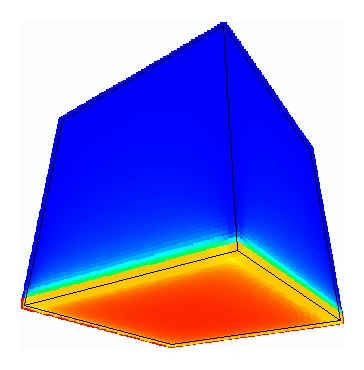
\includegraphics[width=0.72\linewidth]{heat3d_cube.png}
  \caption[Render 3D pola temperatury]{Render 3D pola temperatury dla dziedziny \num{64}$^3$, wykonany wbudowanym rendererem wokselowym programu z~modułu \texttt{ImageUtils.chpl} i~pokazany pod~kątem od~strony gorącej ściany. Widoczna jest podtrzymywana gorąca ściana \(y=0\) (czerwona, \(T=2\)) oraz gradient na~ścianach bocznych opadający ku~zimnym ścianom (\(T=1\)). Barwa odwzorowuje temperaturę w~przedziale \([1,2]\) zgodnie z~mapą HSV od~błękitu do~czerwieni.}
  \label{fig:cube3d}
\end{figure}

Opisana architektura, rozproszony zapis fragmentów bez globalnego gromadzenia, ich późniejsza agregacja poza ścieżką krytyczną oraz opcjonalna wizualizacja, oddziela operacje wejścia-wyjścia i komunikację zbiorową od właściwej pętli obliczeniowej. Jedynym elementem komunikacyjnym tej pętli pozostaje wymiana halo omówiona w~\cref{sec:solver}.

\chapter{Metodologia badań}
\label{ch:metodologia}

\section{Scenariusze i metryki}
\label{sec:scenariusze}

\subsection{Scenariusze badawcze}

Badania podzielono na dwie grupy: weryfikację poprawności oraz pomiary wydajności
i~skalowania. Weryfikacja poprawności obejmowała sprawdzenie,
że wynik obliczeń jest niezależny od~liczby locale, na~które rozdzielono dziedzinę, pod~warunkiem
prawidłowej wymiany warstw brzegowych. Jako niezmiennik kontrolny wykorzystano sumę wartości pola
w~stanie końcowym, raportowaną przez program w~wierszu \texttt{final field: min=\ldots{}
max=\ldots{} sum=\ldots}. Ponieważ pole przyjmuje wartości w~przedziale $[1,2]$, a~jego
średnia jest bliska jedności, suma jest w~przybliżeniu równa liczbie komórek siatki.

Pomiary wydajności obejmowały cztery grupy scenariuszy, zestawione w~tabeli~\ref{tab:scenariusze}:
\begin{itemize}
  \item \textbf{skalowanie wątkowe w~obrębie węzła}: jeden locale (\texttt{-nl 1}),
        zmienna liczba wątków $1/2/4/8/16$, przeprowadzone dla kostki $1000^3$ na~węźle
        Pionier-lab8-1 o~20~wątkach.
  \item \textbf{skalowanie wątkowe przy 9 locale}: kostka $1000^3$, ustalona
        liczba locale, zmienna liczba wątków na~locale.
  \item \textbf{skalowanie po~liczbie węzłów}: kostka $1000^3$, $16$ wątków na~locale,
        liczba locale od~1 do~9.
  \item \textbf{skalowanie rozmiaru zadania}: 9 locale, $16$ wątków na~locale,
        krawędź kostki od~$125$ do~$1000$ (a~więc od~$125^3$ do~$1000^3$ komórek).
\end{itemize}

\begin{table}[htbp]
\centering
\caption{Grupy scenariuszy pomiarowych. Liczbę wątków w~pierwszej grupie oznaczono
symbolem $p$, liczbę locale symbolem $L$, a~krawędź kostki symbolem $N$.}
\label{tab:scenariusze}
\small
\begin{tabular}{@{}>{\raggedright\arraybackslash}p{2.8cm}>{\raggedright\arraybackslash}p{3.4cm}>{\raggedright\arraybackslash}p{4.0cm}>{\raggedright\arraybackslash}p{2.8cm}@{}}
\toprule
Scenariusz & Zmienna & Ustalone & Środowisko \\
\midrule
Wątki, $1000^3$       & $p\in\{1{,}2{,}4{,}8{,}16\}$ & $L{=}1$, $N{=}1000$, 10 kroków & węzeł Pionier-lab8-1 (20 wątków) \\
Wątki, 9 locale      & $p\in\{1{,}2{,}4{,}8{,}16\}$ & $L{=}9$, $N{=}1000$, 100 kroków   & klaster (9 węzłów) \\
Węzły                 & $L\in\{1{,}\ldots{,}9\}$ & $p{=}16$, $N{=}1000$, 100 kroków & klaster (9 węzłów) \\
Rozmiar kostki        & $N\in\{125{,}\ldots{,}1000\}$ & $p{=}16$, $L{=}9$, 100 kroków & klaster (9 węzłów) \\
\bottomrule
\end{tabular}
\end{table}

Skalowanie wątkowe w~obrębie węzła i~skalowanie po~węzłach rozdzielono świadomie:
to dwa różne mechanizmy równoległości, współdzielenie pamięci przez
wątki jednego locale oraz rozproszenie danych między locale połączone z~komunikacją sieciową.
Dopiero zestawienie obu perspektyw pozwala zidentyfikować czynnik ograniczający wydajność.

Górny pułap \num{16} wątków w~powyższych scenariuszach wynika z~architektury węzłów oraz
z~domyślnego zachowania warstwy wykonawczej Chapel. Procesor Intel~Core~i7-12700K jest
układem hybrydowym: ma 8~rdzeni wydajnościowych z~wielowątkowością współbieżną, co daje
\num{16} wątków sprzętowych, oraz 4~rdzenie energooszczędne bez wielowątkowości, łącznie
12~rdzeni fizycznych i~20 wątków logicznych. Skrypt uruchomieniowy żąda liczby wątków na~locale
równej wynikowi polecenia \texttt{nproc}, czyli 20. Warstwa qthreads, korzystająca z~biblioteki
hwloc, przy domyślnym ustawieniu \texttt{CHPL\_RT\_USE\_PU\_KIND=performance} wykorzystuje jednak
wyłącznie jednostki wykonawcze rdzeni wydajnościowych i~pomija rdzenie energooszczędne, co na~tych
węzłach daje \num{16} dostępnych wątków logicznych. Żądanie 20~wątków przekracza tę liczbę, więc
warstwa wykonawcza ogranicza ją do~\num{16} i~zgłasza komunikat \texttt{Reduced
numThreadsPerLocale=20 to 16 to prevent oversubscription}~\cite{chapel-docs}. Każdy węzeł pracuje
zatem efektywnie na~\num{16} wątkach i~tę wartość ustalono we~wszystkich przebiegach wielowęzłowych.

Z~tego samego powodu skalowanie wątkowe w~obrębie węzła prowadzono w~potęgach dwójki
$1/2/4/8/16$. Kolejne podwojenia dają równomiernie rozmieszczone punkty na~osi logarytmicznej,
a~górny punkt \num{16} pokrywa się z~pułapem narzuconym przez warstwę wykonawczą oraz z~liczbą
wątków na~locale używaną w~przebiegach wielowęzłowych, dzięki czemu obie serie pozostają
porównywalne. Nie uwzględniono 20~wątków, ponieważ rdzenie energooszczędne są domyślnie pomijane,
a~samo żądanie 20 i~tak jest redukowane do~\num{16}. Nie uwzględniono też 12~wątków
odpowiadających liczbie rdzeni fizycznych, ponieważ warstwa wykonawcza liczy jednostki wykonawcze
rdzeni wydajnościowych wraz z~wielowątkowością, a~nie same rdzenie fizyczne, a~ponadto 12 nie jest
potęgą dwójki. Jedyną zmienną niezależną w~tych scenariuszach była odpowiednio liczba węzłów lub
rozmiar dziedziny.

Wszystkie przebiegi wykorzystują ten sam zestaw parametrów numerycznych. Współczynnik
dyfuzji przyjęto bezwymiarowo $\alpha=\num{0.25}$, a~gorącą warstwę startową o~grubości
\texttt{hotThickness}=\num{2} płaszczyzn inicjalizowano wzdłuż osi~$y$ przy ścianie $y=0$.
Krok czasowy dobierany jest automatycznie z~warunku~\eqref{eq:cfl}, z~zastosowaniem
współczynnika bezpieczeństwa obniżającego krok o~\SI{2}{\percent} poniżej granicy stabilności:
\begin{equation}
  \Delta t = \num{0.98}\cdot\Delta t_{\max},
  \label{eq:dt}
\end{equation}
co dla~najbardziej niekorzystnego modu, o~naprzemiennym znaku między sąsiednimi
węzłami, daje współczynnik wzmocnienia~\eqref{eq:amp} równy $g=\num{-0.96}$. Ujemny
znak oznacza jedynie, że~amplituda tego modu zmienia znak w~każdym kroku, natomiast
warunek $\lvert g\rvert<1$ gwarantuje, że~jej moduł maleje. Błędy nie narastają,
lecz są tłumione, więc schemat pozostaje stabilny mimo błędów zaokrągleń.
Dla~największej badanej kostki $N=1000$ daje to $\Delta t\approx 6{,}55\cdot 10^{-7}$. Liczba kroków
czasowych $K$ zależy od~grupy scenariusza: wynosi \num{10} przy~skalowaniu wątkowym
na~pojedynczym węźle oraz \num{100} w~eksperymentach wielowęzłowych.

\subsection{Metryki}

Podstawową wielkością mierzoną jest \emph{czas wykonania} $T$, rozumiany jako czas trwania
całej pętli czasowej, mierzony zegarem \texttt{computeTimer} w~locale głównym (locale~0).
Ponieważ krok czasowy zawiera barierę synchronizacyjną wymiany halo, wszystkie locale kończą
krok w~tym samym czasie, więc pomiar z~locale głównego jest reprezentatywny dla całego
przebiegu. Czas ten nie obejmuje inicjalizacji, mierzonej osobno zegarem
\texttt{initTimer}.

Na podstawie czasu wykonania zdefiniowano standardowe miary skalowania silnego:
przyspieszenie $S(p)=T(1)/T(p)$ oraz wydajność równoległą $E(p)=S(p)/p$, zdefiniowane już
wzorami~\eqref{eq:speedup} i~\eqref{eq:efficiency}, gdzie $T(1)$ jest czasem wykonania konfiguracji
bazowej z~jednym wątkiem albo jednym locale.
W~roli $p$ dla skalowania wątkowego przyjęto \emph{efektywną} liczbę wątków,
czyli wartość \texttt{maxTaskPar} po~ewentualnym ograniczeniu przez warstwę wątkową, a~nie liczbę
żądaną. Dla oceny wykorzystania sprzętu niezależnie od~rozmiaru zadania posłużono się
\emph{przepustowością} wyrażoną w~miliardach aktualizacji komórek na~sekundę,
\begin{equation}
  \Pi = \frac{N^3 \cdot K}{T \cdot 10^{9}},
  \label{eq:throughput}
\end{equation}
gdzie $N^3 \cdot K$ jest łączną liczbą aktualizacji komórek (wielkość bezwymiarowa),
$T$ jest czasem wykonania w~sekundach, a~czynnik $10^{9}$ jest prefiksem giga
zamieniającym aktualizacje na~giga-aktualizacje. $\Pi$ wyrażone jest
w~giga-aktualizacjach komórek na~sekundę, co odpowiada konwencji metryki GUPS z~systemu
HPC Challenge~\cite{hpcchallenge}. Dla oszacowania roli
komunikacji wprowadzono \emph{udział komunikacji} w~czasie pojedynczego kroku,
\begin{equation}
  \texttt{comm\_frac} = \frac{t_{\text{fluff}}}{t_{\text{fluff}} + t_{\text{compute}}},
  \label{eq:commfrac}
\end{equation}
gdzie $t_{\text{fluff}}$ i~$t_{\text{compute}}$ są uśrednionymi po~krokach czasami wymiany halo
oraz obliczeń. Wielkość \texttt{comm\_frac} przyjmuje wartości bliskie jedności, gdy dominuje komunikacja,
oraz bliskie zeru, gdy dominują obliczenia. Uzupełniająco rejestrowano objętość wymiany halo
w~bajtach na~krok, obliczaną analitycznie przez procedurę \texttt{haloBytesPerStep} jako łączną
liczbę komórek warstw brzegowych wszystkich locale pomnożoną przez rozmiar elementu.

\subsection{Wybór backendu kompilatora}
\label{sec:backend}

Chapel generuje kod wynikowy jedną z~dwóch dróg: przez backend C (\texttt{CHPL\_LLVM=none})
albo przez backend LLVM (\texttt{CHPL\_LLVM=system}). Aby sprawdzić, czy wybór backendu wpływa
na~wydajność w~docelowym środowisku rozproszonym, ten sam program zbudowano w~obu wariantach
i~porównano na~dziewięciu węzłach klastra Pionier. Każdy wariant uruchomiono dziesięciokrotnie
dla kostki $100^3$, przez \num{100} kroków, z~warstwą komunikacyjną mpi-conduit. Backend LLVM
korzystał z~systemowej instalacji LLVM w~wersji 19.1.7. Wyniki zestawiono w~\cref{tab:llvm}.

\begin{table}[htbp]
\centering
\caption{Porównanie backendu kompilatora C (\texttt{CHPL\_LLVM=none}) i~LLVM
(\texttt{CHPL\_LLVM=system}, LLVM 19.1.7) dla kostki $100^3$ na~dziewięciu węzłach klastra
Pionier, \num{100} kroków, \num{10} powtórzeń. Kolumny mediana, średnia, min i~max dotyczą
czasu wykonania, a~kolumny updateFluff i~compute podają medianę czasu danej fazy na~krok.}
\label{tab:llvm}
\small
\begin{tabular}{@{}lrrrrrr@{}}
\toprule
Backend & mediana & średnia & min & max & updateFluff & compute \\
        & [s] & [s] & [s] & [s] & [s/krok] & [s/krok] \\
\midrule
C (\texttt{none}) & \num{20.015} & \num{19.995} & \num{19.883} & \num{20.096} & \num{0.1966} & \num{0.00185} \\
LLVM 19.1.7       & \num{19.910} & \num{19.908} & \num{19.842} & \num{19.962} & \num{0.1955} & \num{0.00185} \\
\bottomrule
\end{tabular}
\end{table}

Mediany czasu wykonania różnią się o~\SI{0.105}{\second}, czyli około \SI{0.5}{\percent}, co
mieści się w~granicach rozrzutu między powtórzeniami. Wyjaśnia tę różnicę rozkład czasu
pojedynczego kroku: wymiana halo zajmuje około \SI{99}{\percent} kroku, a~same obliczenia około
\SI{1}{\percent}, więc udział komunikacji \texttt{comm\_frac} według~\eqref{eq:commfrac} jest
bliski jedności. Backend kompilatora wpływa wyłącznie na~lokalny kod obliczeniowy, którego czas
jest w~obu wariantach praktycznie taki sam i~stanowi niewielką część kroku, dlatego nie przekłada
się na~całkowity czas wykonania.

Z~tego powodu we~wszystkich dalszych pomiarach używano backendu C (\texttt{CHPL\_LLVM=none}),
który w~komunikacyjnie ograniczonym środowisku wielowęzłowym nie powoduje mierzalnej straty
wydajności.

\section{Procedura i narzędzia pomiarowe}
\label{sec:procedura}

\subsection{Procedura pomiarowa}

Każdą konfigurację uruchamiano dziesięciokrotnie, a~jako wartość reprezentatywną przyjmowano \emph{medianę} czasu wykonania. Wybór mediany zamiast średniej arytmetycznej jest istotny:
pojedyncze przebiegi bywają zaburzone przez chwilowe zdarzenia systemowe, takie jak rywalizacja o~rdzenie,
przejściowe ograniczenie taktowania procesora czy aktywność innych procesów, które zawyżają
czas, lecz nie odzwierciedlają właściwości badanej konfiguracji. Mediana jest odporna na takie
wartości odstające, podczas gdy średnia zostaje przez nie zawyżona. Przykładem jest jedna
z~serii jednowęzłowych, w~której trzy z~dziesięciu przebiegów były wolniejsze o~około pół
sekundy (około \SI{5}{\percent} czasu pojedynczego przebiegu) wskutek przejściowego ograniczenia
taktowania. Skutkowało to podwyższonym odchyleniem
standardowym przy praktycznie niezmienionej medianie.

Przebiegi danej serii wykonywano sekwencyjnie, po~jednym naraz, aby uniknąć wzajemnej
rywalizacji o~pamięć i~pasmo. Serie pomiarowe wykonywano zautomatyzowanym skryptem
\path{bench.sh} opisanym w~\cref{sec:uruchamianie}. Wszystkie pomiary wydajności prowadzono na~środowisku Chapel~2.9
z~warstwą komunikacyjną w~wariancie mpi-conduit. Liczbę wątków na~locale ustawiano zmienną
środowiskową \texttt{CHPL\_RT\_NUM\_THREADS\_PER\_LOCALE}.

Konfigurację każdego przebiegu zapisywano bezpośrednio w~logu w~postaci linii
\texttt{[cfg]} opisanych w~\cref{sec:uruchamianie}: skrypt podaje żądaną liczbę wątków i~locale,
a~program efektywną liczbę wątków po~ograniczeniu przez warstwę qthreads. Na~węzłach Pionier
o~20~wątkach sprzętowych liczba efektywna była równa żądanej dla~wszystkich badanych
konfiguracji ($p\le 16$).


\subsection{Narzędzia pomiarowe}

Czasy mierzono wbudowanymi w~język stoperami (\texttt{stopwatch}), opartymi na~zegarze
monotonicznym wysokiej rozdzielczości o~praktycznej rozdzielczości pojedynczych
mikrosekund, osobno dla inicjalizacji, całej pętli czasowej oraz, w~każdym kroku,
dla wymiany halo, obliczeń i~zapisu. Objętość i~liczbę operacji komunikacyjnych GET, PUT, zdalnych i~atomowych rejestrowano za~pomocą modułu diagnostyki komunikacji GASNet,
włączanego przełącznikiem \texttt{commLog}. Wypisywany raz wiersz \texttt{[comm]} podaje
analityczną objętość wymiany halo na~krok. Zużycie pamięci procesu kontrolowano narzędziem
systemowym \texttt{/usr/bin/time -v}, odczytując maksymalny rezydentny zbiór stron
(ang.~\emph{Resident Set Size}, RSS), co pozwoliło ustalić
graniczne rozmiary kostek mieszczące się w~pamięci danego węzła.

Przetwarzanie zebranych logów oraz rysowanie wykresów zrealizowano skryptami w~języku Python
z~biblioteką \texttt{matplotlib}. Podstawową formą prezentacji jest wykres pudełkowy
rozkładu czasu wykonania z~naniesionymi punktami poszczególnych przebiegów, medianą
oraz średnią. Uzupełniają go wykresy metryk pochodnych: przyspieszenia, wydajności,
przepustowości i~udziału komunikacji. Taka forma pokazuje jednocześnie środek rozkładu
i~rozrzut, co jest istotne przy ocenie powtarzalności.

Do diagnozy zachowania sieci wykorzystano dedykowany skrypt sondujący, który równocześnie
obciąża łącze strumieniem \texttt{iperf3} w~trybie UDP o~przepływności zbliżonej do~granicy
łącza oraz monitoruje straty pakietów z~kilku niezależnych perspektyw: procentu utraconych
pakietów ICMP, przyrostów liczników odrzuceń na~lokalnym interfejsie sieciowym oraz, co
najważniejsze, przyrostów liczników błędów bufora odbiorczego UDP po~stronie odbiorcy
(\texttt{InErrors}, \texttt{RcvbufErrors}). Rosnące błędy bufora odbiorczego pod~obciążeniem są
bezpośrednim dowodem przeciążenia typu \emph{incast}, które w~wariancie AMUDP prowadzi do~awarii
typu \texttt{ECONGESTION}~\cite{incast}. Narzędzie to pozwoliło odróżnić przyczyny sieciowe od~obliczeniowych
i~dyskowych oraz uzasadnić wybór wariantu transportu opartego na~protokole TCP.

\subsection{Przykład wyznaczenia metryk}

Dla uporządkowania powyższych definicji poniżej przedstawiono sposób wyznaczenia metryk pochodnych na~jednym
scenariuszu. Rozważono skalowanie wątkowe kostki $1000^3$ na~węźle Pionier o~20~wątkach. Jednowątkowa
konfiguracja bazowa osiągnęła medianę czasu wykonania $T(1)=\SI{9.812}{\second}$, natomiast
optymalna konfiguracja ośmiowątkowa $T(8)=\SI{8.094}{\second}$. Zgodnie z~\eqref{eq:speedup}
przyspieszenie wynosi $S(8)=9{,}812/8{,}094\approx\num{1.212}$, a~wydajność równoległa według
\eqref{eq:efficiency}, $E(8)=1{,}212/8\approx\num{0.152}$. Przepustowość dla tej konfiguracji, przy
$K=10$ krokach, obliczono z~\eqref{eq:throughput}: $1000^3\cdot 10 = 10^{10}$ aktualizacji komórek
w~czasie $T(8)=\SI{8.094}{\second}$ daje $10^{10}/8{,}094 \approx \num{1.24}\cdot 10^{9}$ aktualizacji
na~sekundę, a~po~podzieleniu przez $10^{9}$ (prefiks giga) $\Pi \approx \num{1.24}$ miliarda
aktualizacji komórek na~sekundę.
Zabieg ten powtórzono dla każdej konfiguracji każdego scenariusza, dzięki czemu wszystkie wykresy
i~zestawienia w~\cref{ch:wyniki} opierają się na~jednolicie zdefiniowanych wielkościach.

\subsection{Kontrola warunków i~zagrożenia dla trafności}

Wiarygodność wniosków zależy od~kontroli czynników zakłócających. W~toku badań zidentyfikowano
i~ograniczono kilka takich czynników.

Zmienność środowiska pochodzi ze~współdzielenia maszyny z~innymi procesami oraz dynamicznego
zarządzania taktowaniem procesora, co wprowadza zmienność czasu wykonania. Ograniczono ją przez
sekwencyjne uruchamianie przebiegów, dziesięciokrotne powtórzenia oraz stosowanie mediany. Tam,
gdzie mimo to pojawiły się wartości odstające, czyli pojedyncze wolniejsze przebiegi wskutek przejściowego
ograniczenia taktowania, fakt ten odnotowano jawnie i~potraktowano jako artefakt pomiaru, a~nie
własność konfiguracji.

Nierówny podział dziedziny pojawia się, gdy liczba locale nie dzieli równo boku kostki $1000^3$.
Powoduje to nierównomierne obciążenie i~zaburza gładkość krzywej skalowania. Nie jest to
błąd pomiaru, lecz rzeczywista własność dekompozycji. Uwzględniono ją w~interpretacji
niemonotonicznego przebiegu skalowania po~węzłach.

Trafność zewnętrzna wyników jest ograniczona: uzyskano je na~konkretnym, niewielkim klastrze z~siecią
\SI{1}{\giga\bit\per\second}. Wartości bezwzględne nie przenoszą się wprost na~inne środowiska. Wnioski mają
jednak charakter ogólny i~wynikają z~właściwości samych obliczeń stencilowych:
obliczenia te są ograniczone przepustowością pamięci oraz komunikacją sieciową, a~większe
zadania lepiej wykorzystują klaster~\cite{roofline,datta-stencil}.

\chapter{Wyniki i analiza}
\label{ch:wyniki}

\section{Poprawność i wydajność wariantów}
\label{sec:poprawnosc-wydajnosc}

Główny wariant programu zarządza buforami operatorem zamiany \texttt{<=>}.
Rozważono też wariant naprzemiennego buforowania (ping-pong). Ponieważ oba nie
różnią się znacząco wydajnością, dalsze wyniki dotyczą wariantu głównego
z~operatorem zamiany.

\subsection{Weryfikacja poprawności numerycznej}
\label{subsec:poprawnosc}

Przed przystąpieniem do jakichkolwiek pomiarów wydajnościowych konieczne było
ustanowienie wiarygodnego kryterium poprawności obliczeń. Bez takiego kryterium
przyspieszenie z~równoległości nie ma znaczenia, łatwo
bowiem uzyskać krótszy czas wykonania kosztem cichego naruszenia poprawności
wyniku. W~przypadku badanego programu przyjęto niezmiennik oparty na
własnościach pola temperatury oraz na jego całkowitej sumie.

Warunki początkowe i~brzegowe zadania dobrano tak, aby rozwiązanie pozostawało
przez cały czas symulacji ograniczone do przedziału $[1,2]$. Program po
zakończeniu obliczeń raportuje statystyki końcowego pola w~postaci wpisu
\texttt{final field: min=1.0 max=2.0 sum=<S>}. Utrzymanie dolnej granicy
\num{1.0} oraz górnej granicy \num{2.0} jest bezpośrednią konsekwencją zasady
maksimum dla równania przewodnictwa cieplnego: schemat jawny z~odpowiednio
dobranym krokiem czasowym nie może wygenerować wartości spoza zakresu
wyznaczonego przez dane początkowe i~brzegowe. Naruszenie któregokolwiek
z~tych ograniczeń natychmiast sygnalizowałoby błąd implementacji schematu
różnicowego lub niestabilność numeryczną.

Kluczową rolę w~weryfikacji odgrywa jednak suma wszystkich elementów pola,
w~przybliżeniu równa liczbie komórek siatki. Jednocześnie suma $S$ dobrze
oddaje stan całej dziedziny i~szybko reaguje na~różnice między konfiguracjami:
najmniejsze rozejście się wyników widać jako rozbieżność sum.

Właśnie na tej podstawie zweryfikowano poprawność obliczeń wielowęzłowych.
Przebieg uruchomiony na pojedynczym locale (\texttt{-nl 1}) daje pewną wartość
sumy odniesienia. Ten sam problem rozdzielony na $N$~locale daje identyczną
sumę \emph{pod warunkiem}, że po każdym kroku czasowym wykonywana jest
wymiana warstw brzegowych (halo) za pomocą operacji \texttt{updateFluff}.
Pominięcie tej wymiany skraca czas wykonania, lecz suma $S$ zaczyna się
rozchodzić względem wartości odniesienia. Wynik staje się \emph{cicho błędny}.
W~przeprowadzonych pomiarach (dziedzina $1000^3$, 100 kroków) suma końcowa pola
wynosiła $1{,}00518\cdot 10^{9}$ i~była identyczna dla każdej liczby lokacji od~1 do~9
(po dziesięć powtórzeń na~konfigurację), co empirycznie potwierdza niezależność
wyniku od~dekompozycji dziedziny.
Wymiana warstw brzegowych
jest więc niezbędna do~poprawności i~nie da się jej pominąć dla zysku
wydajności. Suma jest przy tym
miarą odporną na~błędy systematyczne, do~jakich należy pominięcie wymiany halo,
które rozchodzi pole w~jednym kierunku, a~nie na~błędy kompensujące się.
Zasada maksimum ogranicza każdą komórkę do~przedziału $[1,2]$, więc punktowe
naruszenie tej granicy zostałoby wychwycone niezależnie od sumy. Ta obowiązkowa
komunikacja, jak pokazano w~\cref{sec:skalowanie-komunikacja}, jest głównym wąskim
gardłem systemu.


\subsection{Skalowanie wątkowe na pojedynczym węźle}
\label{subsec:skalowanie-watkowe}

W~tej części przeanalizowano wydajność jednowęzłową. Celem tej serii eksperymentów
było zbadanie, jak czas wykonania programu zależy od liczby wątków obliczeniowych
przy ustalonym rozmiarze zadania, a~zatem ile faktycznie zyskuje się na
zrównolegleniu wewnątrzwęzłowym. Pomiary wykonano dla dziedziny $1000^3$ na~węźle klastra Pionier.

\Cref{tab:threads-1000} przedstawia wyniki tego eksperymentu. Faktyczna liczba
zadań qthreads jest tu równa liczbie żądanej.

\begin{table}[htbp]
\centering
\caption{Skalowanie wątkowe na pojedynczym węźle, dziedzina $1000^3$,
\texttt{-nl 1}, \num{10} kroków $\times$ \num{10} powtórzeń, Chapel 2.9,
kanał MPI, węzeł Pionier.}
\label{tab:threads-1000}
\begin{tabular}{rrrrrrrrr}
\toprule
Żądane & \texttt{maxTaskPar} & Mediana & Średnia & Min. & Maks. & Odch. std. & $S$ & $E$ \\
wątki & & [s] & [s] & [s] & [s] & [s] & & \\
\midrule
\num{1}  & \num{1}  & \num{9.812} & \num{9.814} & \num{9.803} & \num{9.829} & \num{0.008} & \num{1.000} & \num{1.000} \\
\num{2}  & \num{2}  & \num{9.948} & \num{10.104} & \num{9.941} & \num{10.470} & \num{0.240} & \num{0.986} & \num{0.493} \\
\num{4}  & \num{4}  & \num{8.362} & \num{8.362} & \num{8.356} & \num{8.365} & \num{0.003} & \num{1.173} & \num{0.293} \\
\num{8}  & \num{8}  & \num{8.094} & \num{8.095} & \num{8.087} & \num{8.101} & \num{0.004} & \num{1.212} & \num{0.152} \\
\num{16} & \num{16} & \num{8.739} & \num{8.741} & \num{8.731} & \num{8.763} & \num{0.008} & \num{1.123} & \num{0.070} \\
\bottomrule
\end{tabular}
\end{table}

Obraz jest tu jakościowo odmienny i~znacznie korzystniejszy. Przejście z~jednego do
dwóch wątków nie przynosi niemal zysku: mediana rośnie z~\SI{9.812}{\second} do
\SI{9.948}{\second}, a~trzy z~dziesięciu przebiegów dwuwątkowych były wyraźnie
wolniejsze, około \SI{10.47}{\second}, wskutek przejściowego ograniczenia taktowania.
Dopiero cztery wątki dają wyraźny skok wydajności: mediana spada do
\SI{8.362}{\second} (przyspieszenie \num{1.173}), a~optimum osiągane jest przy
ośmiu wątkach (\SI{8.094}{\second}, przyspieszenie \num{1.212}). Dalsze zwiększanie
liczby wątków ponownie szkodzi: przy szesnastu czas rośnie do
\SI{8.739}{\second}. Maksymalne uzyskane przyspieszenie wynosi zatem tylko około
\num{1.21}$\times$, mimo dostępności dwudziestu wątków.

Wydajność $E$ spada przy tym bardzo ostro: z~\num{1.000}
przez \num{0.493} i~\num{0.293} aż do \num{0.070} przy szesnastu wątkach. Tak
gwałtowny spadek to typowy objaw problemu
\emph{ograniczonego pasmem pamięci}~\cite{datta-stencil}. Schemat różnicowy jest operacją o~niskiej intensywności arytmetycznej, więc jego
przepustowość limituje pasmo pamięci głównej, a~nie liczba dostępnych rdzeni.
Po~nasyceniu tego pasma dodatkowe wątki rywalizują o~tę samą magistralę, co~prowadzi
do~degradacji wydajności.

Zwiększanie liczby wątków ponad pewien próg nie pomaga tu, a~wręcz szkodzi: po~nasyceniu
magistrali pamięci dodatkowe wątki nie znajdują użytecznej pracy.
\Cref{fig:threads-1000} ilustruje te zależności: lewy panel
przedstawia rozkład czasów wykonania w~postaci wykresu pudełkowego, a~prawy
zestawia zmierzone przyspieszenie z~przyspieszeniem idealnym oraz z~krzywą
wydajności, uwidaczniając odejście od skalowania liniowego już przy dwóch
wątkach.

\begin{figure}[htbp]
\centering
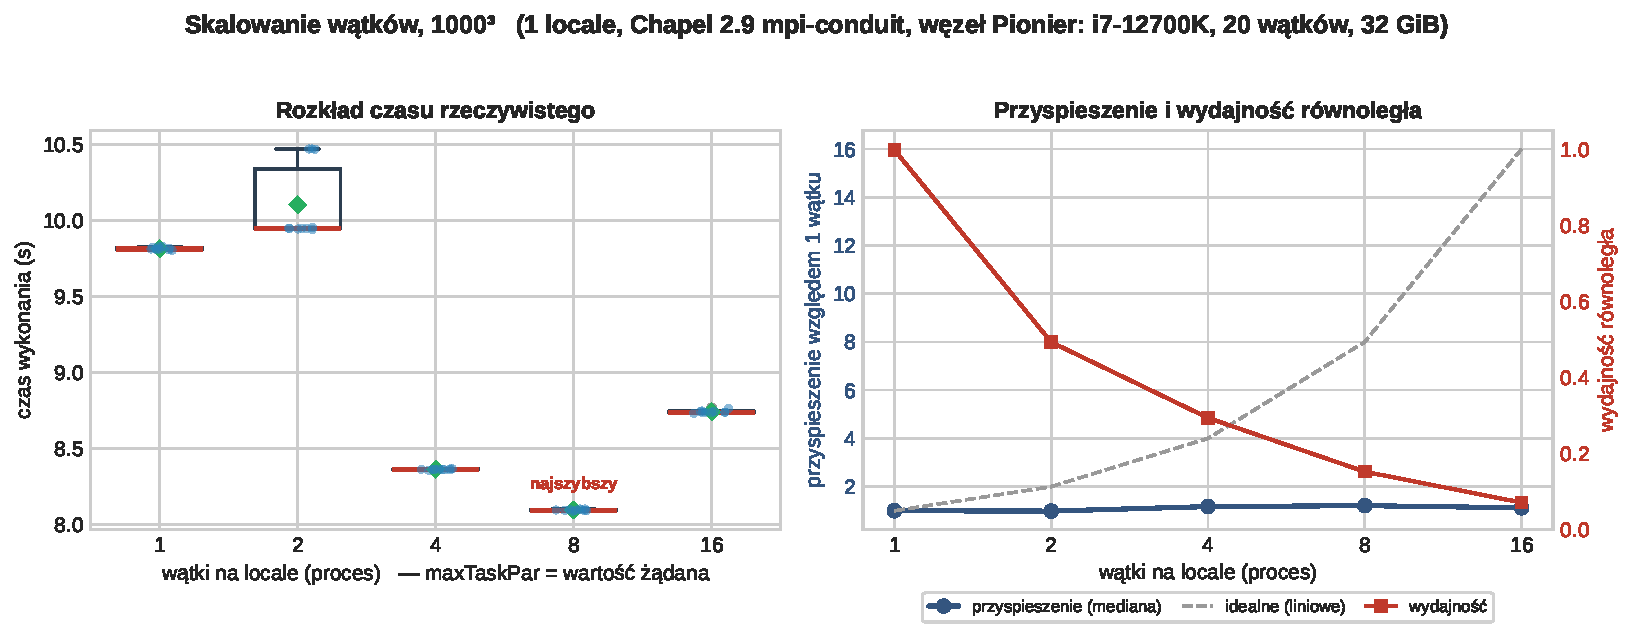
\includegraphics[width=0.95\linewidth]{threads_1000.pdf}
\caption{Skalowanie wątkowe dla dziedziny $1000^3$ na węźle Pionier.
Lewy panel: rozkład czasu wykonania w~postaci wykresu pudełkowego w~funkcji liczby
wątków. Prawy panel: zmierzone przyspieszenie na tle przyspieszenia idealnego
oraz wydajność $E$.}
\label{fig:threads-1000}
\end{figure}

W~części jednowęzłowej równoległość wątkowa przynosi w~najlepszym
razie skromny, około dwudziestoprocentowy zysk, a~wydajność szybko załamuje się
wraz ze wzrostem liczby wątków. Bezpośrednią przyczyną jest ograniczenie
pasmem pamięci. Sytuacja ta pogłębia się dopiero przy skalowaniu na~wiele węzłów.

\section{Skalowanie i ograniczenia komunikacji}
\label{sec:skalowanie-komunikacja}

W~tej części przeanalizowano zachowanie programu przy rozdzieleniu obliczeń na wiele
węzłów klastra połączonych siecią Ethernet \SI{1}{\giga\bit\per\second}.
Eksperymenty w~tej sekcji przeprowadzono na klastrze dla dziedziny $1000^3$
i~\num{100} kroków czasowych. Wykazano, że badany system jest \emph{ograniczony
komunikacją}: to przepustowość sieci, a~nie moc obliczeniowa węzłów, wyznacza
pułap osiąganej wydajności.

\subsection{Skalowanie liczbą węzłów}
\label{subsec:skalowanie-wezly}

\Cref{tab:node-scaling} przedstawia czas wykonania w~funkcji liczby węzłów, od
jednego do dziewięciu, dla dziedziny $1000^3$. Oprócz statystyk czasu podano
przyspieszenie, wydajność oraz objętość danych wymienianych w~ramach warstw
brzegowych na jeden krok czasowy w~kolumnie ,,Bajty/krok''.

\begin{table}[htbp]
\centering
\caption{Skalowanie liczbą węzłów, dziedzina $1000^3$, \num{100} kroków.}
\label{tab:node-scaling}
\begin{tabular}{lrrrrrrr}
\toprule
Węzły & Mediana & Średnia & Min. & Odch. std. & $S$ & $E$ & Bajty/krok \\
& [s] & [s] & [s] & [s] & & & \\
\midrule
\num{1}  & \num{87.344} & \num{87.307} & \num{87.104} & \num{0.092} & \num{1.000} & \num{1.000} & \num{0} \\
\num{2}  & \num{51.943} & \num{51.957} & \num{51.858} & \num{0.107} & \num{1.682} & \num{0.841} & \num{16000000} \\
\num{3}  & \num{52.978} & \num{53.413} & \num{52.862} & \num{1.316} & \num{1.649} & \num{0.550} & \num{32000000} \\
\num{4}  & \num{36.670} & \num{36.889} & \num{36.203} & \num{0.894} & \num{2.382} & \num{0.595} & \num{32032000} \\
\num{5}  & \num{41.476} & \num{41.482} & \num{41.347} & \num{0.093} & \num{2.106} & \num{0.421} & \num{64000000} \\
\num{6}  & \num{32.240} & \num{32.243} & \num{32.076} & \num{0.115} & \num{2.709} & \num{0.452} & \num{48064000} \\
\num{7}  & \num{37.114} & \num{37.112} & \num{36.909} & \num{0.156} & \num{2.353} & \num{0.336} & \num{96000000} \\
\num{8}  & \num{42.941} & \num{42.909} & \num{42.419} & \num{0.198} & \num{2.034} & \num{0.254} & \num{48096064} \\
\num{9}  & \num{36.832} & \num{36.817} & \num{36.469} & \num{0.157} & \num{2.371} & \num{0.263} & \num{64128000} \\
\bottomrule
\end{tabular}
\end{table}

Skalowanie węzłowe okazuje się wyraźnie \emph{niemonotoniczne}. Zamiast
oczekiwanego, systematycznego spadku czasu wraz ze wzrostem liczby węzłów,
obserwuje się silny ,,ząbek'' pomiędzy parzystymi a~nieparzystymi liczbami
węzłów. Najlepszy wynik uzyskano dla sześciu węzłów (mediana
\SI{32.240}{\second}, przyspieszenie \num{2.709}), podczas gdy sąsiednie
konfiguracje pięcio- i~siedmiowęzłowa wypadają zauważalnie gorzej
(\SI{41.476}{\second} oraz \SI{37.114}{\second}). Źródłem tego zjawiska jest
nierównomierny podział dziedziny $1000^3$: gdy liczba węzłów nie dzieli
gładko boku kostki, powstaje niezrównoważenie obciążenia, w~którym niektóre węzły
otrzymują większe poddziedziny i~stają się elementem spowalniającym całość,
co dodatkowo splata się ze wzrostem objętości komunikacji między węzłami.

Niezależnie od tych oscylacji, obraz ogólny jest jednoznaczny:
przyspieszenie \emph{płaszczy się} na poziomie około \num{2.4}$\times$ i~nie
zbliża się do skalowania liniowego, mimo dziewięciokrotnego zwiększenia liczby
węzłów~\cite{amdahl}. Wydajność spada z~\num{1.000} do zaledwie \num{0.263}
przy dziewięciu węzłach. Kluczem do wyjaśnienia jest ostatnia kolumna tabeli:
objętość wymienianych warstw brzegowych rośnie w~przybliżeniu liniowo wraz
z~liczbą węzłów, od \num{0} bajtów dla pojedynczego węzła, w~którym nie ma komunikacji
międzywęzłowej, do ponad \num{64000000} bajtów na krok przy dziewięciu węzłach.
Każdy dodany węzeł wnosi pewną moc obliczeniową, lecz zarazem powiększa
całkowity ruch sieciowy, a~przy powolnym łączu ten drugi efekt szybko
pochłania korzyść z~pierwszego. System jest zatem ograniczony komunikacją.

\begin{figure}[htbp]
\centering
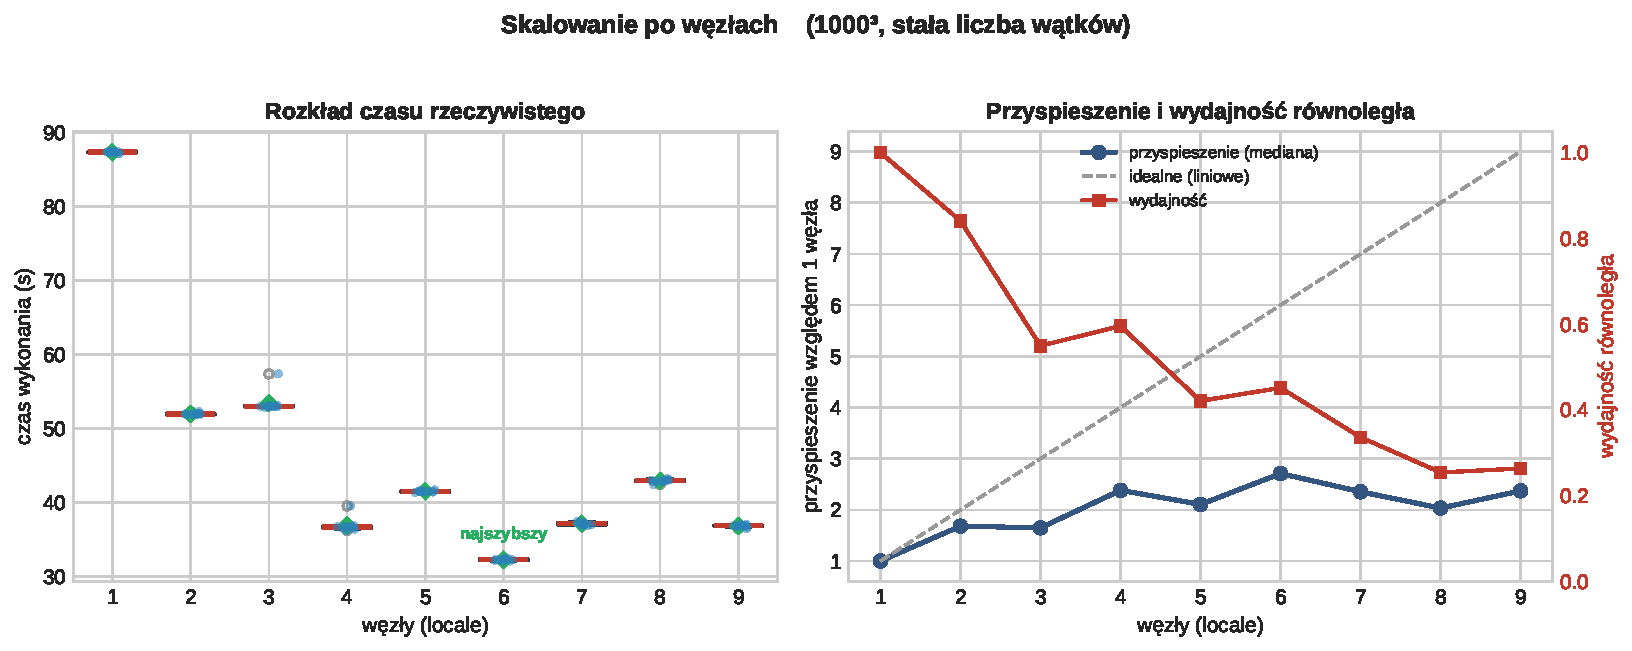
\includegraphics[width=0.95\linewidth]{node_scaling.pdf}
\caption{Skalowanie liczbą węzłów dla dziedziny $1000^3$. Lewy panel: rozkład
czasu wykonania w~funkcji liczby węzłów. Prawy panel: przyspieszenie na tle
przyspieszenia idealnego oraz wydajność $E$.}
\label{fig:node-scaling}
\end{figure}

\begin{figure}[htbp]
\centering
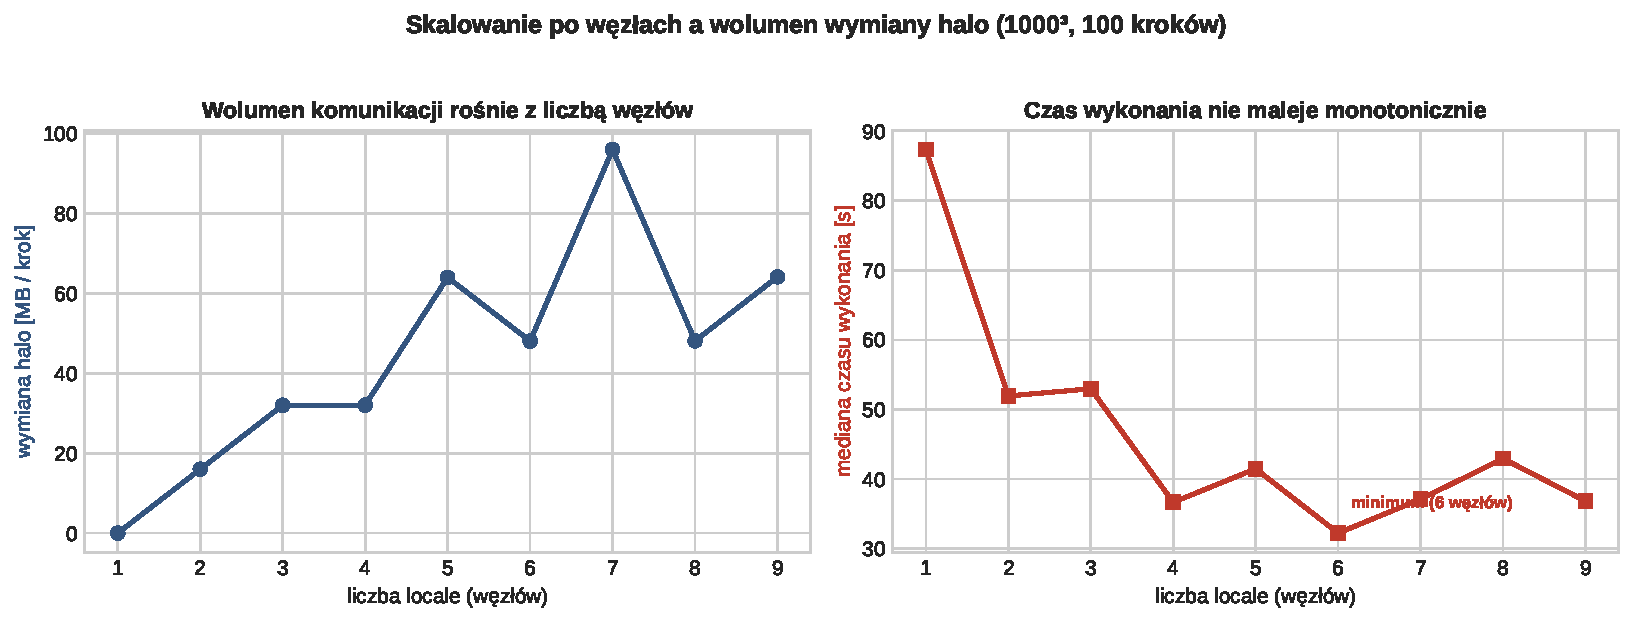
\includegraphics[width=0.95\linewidth]{bytes_vs_nodes.pdf}
\caption{Objętość warstw brzegowych wymienianych na krok w~megabajtach oraz
mediana czasu wykonania w~funkcji liczby węzłów.}
\label{fig:bytes-vs-nodes}
\end{figure}

Zależności te zilustrowano na \cref{fig:node-scaling} oraz \cref{fig:bytes-vs-nodes}.
Pierwszy z~nich uwidacznia zarówno oscylacyjny charakter czasu wykonania, jak
i~znaczne odejście krzywej przyspieszenia od ideału liniowego. Drugi zestawia
rosnącą objętość komunikacji z~czasem wykonania, czyniąc bezpośrednio widocznym
związek między nasilającym się ruchem sieciowym a~stagnacją wydajności.

\subsection{Skalowanie wątkowe przy dziewięciu węzłach}
\label{subsec:skalowanie-watki-9n}

Aby rozstrzygnąć, czy wąskim gardłem w~konfiguracji wielowęzłowej jest
komunikacja, czy może niedostateczne wykorzystanie rdzeni w~obrębie węzła,
powtórzono skalowanie wątkowe przy ustalonej liczbie dziewięciu węzłów.
Wyniki zawiera \cref{tab:threads-9n}.

\begin{table}[htbp]
\centering
\caption{Skalowanie wątkowe przy dziewięciu węzłach, dziedzina $1000^3$,
\num{100} kroków.}
\label{tab:threads-9n}
\begin{tabular}{lrrrrrr}
\toprule
Konfiguracja & Mediana & Średnia & Min. & Odch. std. & $S$ & Obl./krok \\
& [s] & [s] & [s] & [s] & & [s] \\
\midrule
1 wątek   & \num{34.003} & \num{34.245} & \num{33.805} & \num{0.740} & \num{1.000} & \num{0.1422} \\
2 wątki   & \num{35.217} & \num{35.252} & \num{33.715} & \num{1.184} & \num{0.966} & \num{0.1481} \\
4 wątki   & \num{32.563} & \num{32.850} & \num{32.090} & \num{1.086} & \num{1.044} & \num{0.1600} \\
8 wątków  & \num{34.694} & \num{34.616} & \num{34.215} & \num{0.245} & \num{0.980} & \num{0.1775} \\
16 wątków & \num{36.623} & \num{36.633} & \num{36.208} & \num{0.195} & \num{0.928} & \num{0.1982} \\
\bottomrule
\end{tabular}
\end{table}

Odpowiedź jest jednoznaczna. Czas wykonania pozostaje niemal płaski w~zakresie
od około \num{32} do \num{37} sekund niezależnie od liczby wątków, z~płytkim
minimum przy czterech wątkach (\SI{32.563}{\second}). Przyspieszenie oscyluje
wokół jedności i~nigdy nie przekracza \num{1.044}. Najbardziej wymowna jest
jednak kolumna średniego czasu obliczeń na krok: rośnie ona
\emph{monotonicznie} wraz z~liczbą wątków, od \SI{0.1422}{\second} przy jednym
wątku do \SI{0.1982}{\second} przy szesnastu. Gdyby problem był ograniczony mocą
obliczeniową, dodawanie wątków skracałoby czas obliczeń na krok. Obserwuje się
jednak zjawisko przeciwne: czas ten rośnie. Nie jest to skutek nadmiernej liczby
wątków względem rdzeni, bo~te pozostają wolne ($p\le 16\le 20$), lecz rywalizacji
o~zasoby współdzielone: dodatkowe wątki nie znajdują użytecznej pracy, lecz
konkurują o~pasmo pamięci oraz z~wątkiem odpytującym warstwę komunikacyjną
GASNet~\cite{gasnet-spec}. Zwiększanie liczby wątków nie pomaga, ponieważ problem
jest ograniczony komunikacją, a~nie obliczeniami. \Cref{fig:threads-9n}
przedstawia te zależności graficznie.

\begin{figure}[htbp]
\centering
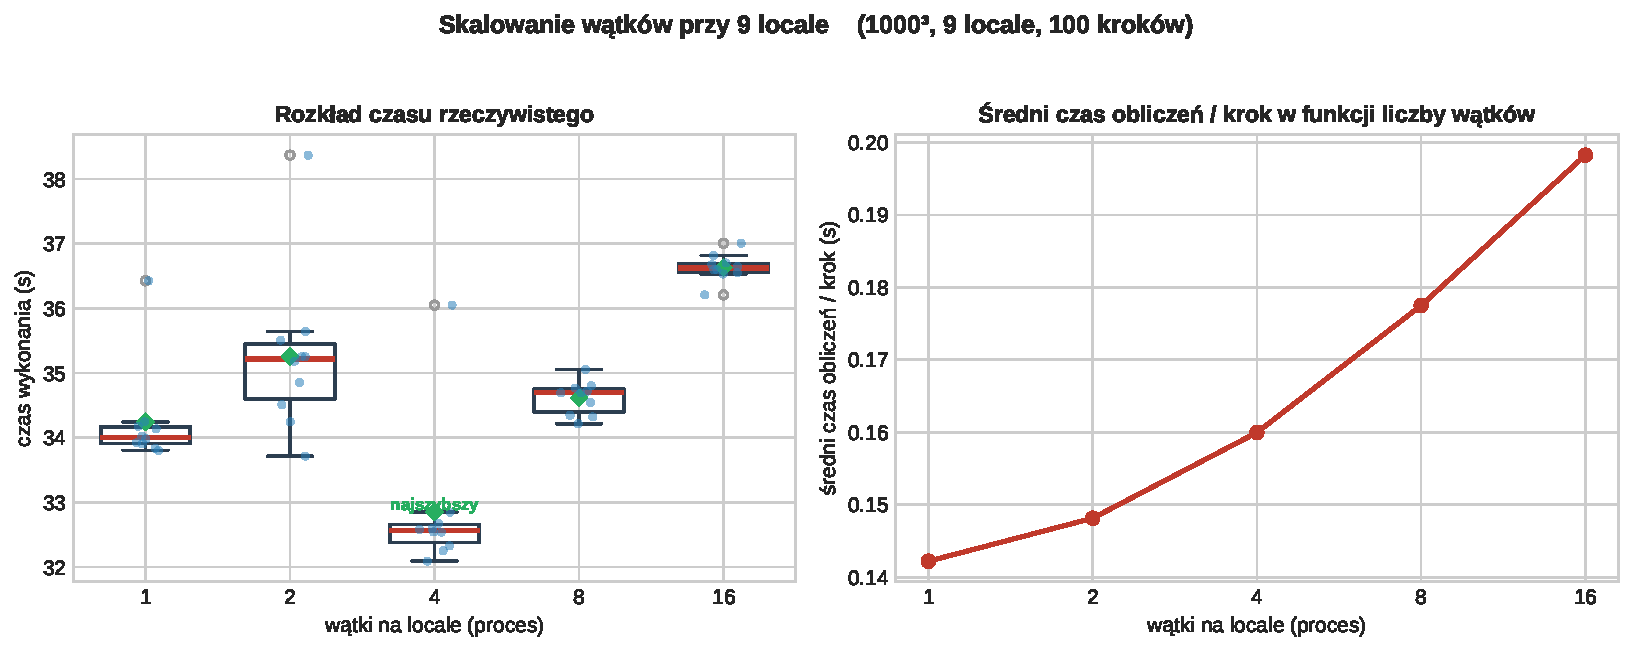
\includegraphics[width=0.95\linewidth]{threads_9nodes.pdf}
\caption{Skalowanie wątkowe przy dziewięciu węzłach, dziedzina $1000^3$.
Lewy panel: rozkład czasu wykonania. Prawy panel: średni czas obliczeń na krok
w~funkcji liczby wątków, rosnący wskutek rywalizacji o~zasoby współdzielone.}
\label{fig:threads-9n}
\end{figure}

\subsection{Skalowanie rozmiaru zadania}
\label{subsec:skalowanie-rozmiar}

Ostatni zestaw eksperymentów bada wpływ rozmiaru dziedziny na wydajność przy
ustalonej liczbie dziewięciu węzłów. \Cref{tab:cube-size} zestawia czasy
wykonania, przepustowość wyrażoną w~miliardach komórek na sekundę
(mld komórek/s) oraz udział komunikacji \texttt{comm\_frac}~\eqref{eq:commfrac}.

\begin{table}[htbp]
\centering
\caption{Skalowanie rozmiaru dziedziny przy dziewięciu węzłach, \num{100}
kroków.}
\label{tab:cube-size}
\begin{tabular}{lrrrr}
\toprule
Rozmiar & Mediana & Średnia & Przepustowość & \texttt{comm\_frac} \\
& [s] & [s] & [mld komórek/s] & \\
\midrule
$125^3$  & \num{1.668}   & \num{1.670}   & \num{0.117} & \num{0.963} \\
$250^3$  & \num{2.640}   & \num{2.652}   & \num{0.592} & \num{0.947} \\
$500^3$  & \num{7.625}   & \num{7.673}   & \num{1.639} & \num{0.729} \\
$1000^3$ & \num{36.741}  & \num{36.802}  & \num{2.722} & \num{0.454} \\
\bottomrule
\end{tabular}
\end{table}

Wynik ten najlepiej potwierdza, że ograniczenie ma charakter komunikacyjny.
Przepustowość rośnie systematycznie wraz z~rozmiarem dziedziny, od zaledwie
\SI{0.117}{} mld komórek/s dla najmniejszej kostki $125^3$ do \SI{2.722}{} mld komórek/s
dla największej kostki $1000^3$. Jednocześnie udział komunikacji
\texttt{comm\_frac} maleje monotonicznie z~\num{0.963} do \num{0.454}. Innymi
słowy, dla małych dziedzin blisko \SI{96}{\percent} czasu pochłania
komunikacja, a~faktyczne obliczenia stanowią margines. Wraz ze~wzrostem dziedziny
proporcje te wyrównują się i~przy~$1000^3$ komunikacja oraz obliczenia zajmują już
zbliżony czas. Nawet przy największej zbadanej kostce
komunikacja wciąż odpowiada za~blisko połowę czasu kroku. Trend jest wprawdzie
korzystny, lecz w~osiągalnym zakresie rozmiarów zadanie nie przestaje być istotnie
obciążone komunikacją.

Mechanizm tego zjawiska jest geometryczny: objętość dziedziny rośnie jak~$N^3$,
a~powierzchnia warstw brzegowych
jak~$N^2$, więc wraz ze wzrostem $N$ poprawia się stosunek pracy obliczeniowej
do~komunikacji. Duże kostki znacznie lepiej wykorzystują klaster niż małe,
zdominowane przez narzut komunikacyjny.

Rozmiar wymiany halo zależy od~geometrycznego układu dekompozycji. Dla
zilustrowania rozważmy dwuwymiarową dziedzinę $100\times 100$ podzieloną na cztery
lokale. Przy podziale plastrami wzdłuż jednej osi każdy blok ma wymiary
$25\times 100$, dwa skrajne lokale wysyłają po $100$ komórek brzegowych, a~dwa
wewnętrzne po $200$, co daje łącznie $600$ komórek wymienianych na krok. Przy
podziale na bloki kwadratowe $50\times 50$ każdy z~czterech lokali wysyła do
dwóch sąsiadów brzeg poziomy i~pionowy po $50$ komórek, co daje
$4\cdot(50+50)=400$ komórek. W~obu przypadkach objętość wymiany jest rzędu pola
powierzchni granicy, a~nie objętości, co w~trzech wymiarach przekłada się na
omówioną zależność $N^2$.

Największą zbadaną dziedziną jest $1000^3$. Omówione zależności ilustruje \cref{fig:cube-size}.

\begin{figure}[htbp]
\centering
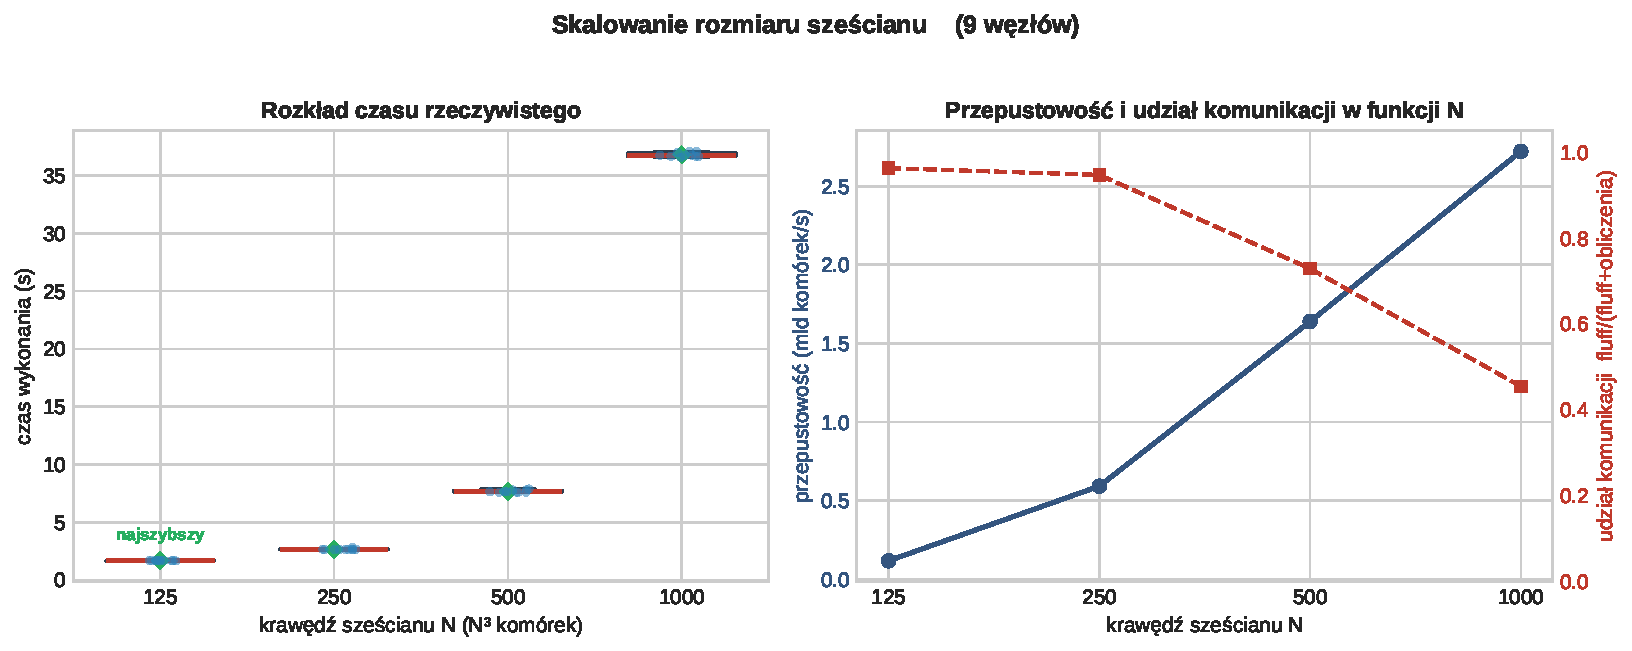
\includegraphics[width=0.95\linewidth]{cube_size.pdf}
\caption{Skalowanie rozmiaru dziedziny przy dziewięciu węzłach. Lewy panel:
rozkład czasu wykonania dla kolejnych rozmiarów. Prawy panel: przepustowość
oraz udział komunikacji \texttt{comm\_frac} w~funkcji rozmiaru kostki.}
\label{fig:cube-size}
\end{figure}

\subsection{Synteza: system ograniczony komunikacją}
\label{subsec:synteza-comm}

Wyniki z tego rozdziału wskazują wspólnie, że system jest ograniczony
komunikacją i~przepustowością pamięci, a~nie mocą obliczeniową. Przyspieszenie
węzłowe płaszczy się na poziomie około \num{2.4}$\times$ (\cref{tab:node-scaling}),
daleko od skalowania liniowego, mimo dziewięciokrotnego zwiększenia liczby
węzłów. Zwiększanie liczby wątków na~węzeł nie przynosi poprawy, a~w~konfiguracji
wielowęzłowej średni czas obliczeń na~krok wręcz rośnie z~liczbą wątków
(\cref{tab:threads-9n}), co wskazuje na~nasycenie zasobów współdzielonych, a~nie na~niedobór
mocy obliczeniowej. Udział komunikacji dominuje przy małych dziedzinach i~maleje
dopiero dla dużych kostek (\cref{tab:cube-size}), zgodnie z~geometryczną relacją
między objętością $N^3$ a~powierzchnią $N^2$. Na każdym węźle jeden wątek warstwy
komunikacyjnej GASNet obciąża rdzeń w~niemal stu procentach, prowadząc aktywne
odpytywanie (ang.~\emph{busy-polling}) w~oczekiwaniu na~postęp komunikacji, co potwierdzono
analizą stosów wywołań w~debugerze. To nie jest obciążenie obliczeniowe, lecz
widoczny i~mierzalny skutek ograniczenia komunikacją.

Fizycznym ograniczeniem jest łącze Ethernet o~przepustowości
\SI{1}{\giga\bit\per\second}, które dla dziedziny rzędu $1000^3$ ulega
nasyceniu. Objętość warstw brzegowych na krok rośnie zarówno z~liczbą węzłów,
jak i~z~kwadratem boku dziedziny, wobec czego to sieć, a~nie procesory,
wyznacza pułap wydajności.

Osobnego omówienia wymaga dobór kanału komunikacyjnego GASNet, który okazał
się decydujący dla tego, czy obliczenia w~ogóle kończą się poprawnie~\cite{gasnet}.
W~pomiarach kanał \texttt{udp} przerywał działanie błędem \texttt{ECONGESTION}
pod obciążeniem typu incast, natomiast kanał \texttt{mpi} kończył obliczenia
poprawnie, choć wolniej. Z~tego powodu nowsza seria pomiarów wykorzystuje kanał
MPI: odporność na~zawodną sieć jest tu ważniejsza od szybkości.

Skoro system jest
ograniczony komunikacją, dalszej poprawy wydajności nie należy szukać ani
w~zwiększaniu liczby wątków, ani w~dokładaniu kolejnych węzłów, lecz przede
wszystkim w~przyspieszeniu warstwy komunikacyjnej, czy to przez zastosowanie
szybszego łącza sieciowego, czy przez wybór wydajniejszego kanału komunikacyjnego GASNet.
Dopóki halo wymieniane jest przez łącze \SI{1}{\giga\bit\per\second}, klaster
wciąż czeka na~dane z~sieci, a~część rdzeni pozostaje niewykorzystana.

\subsection{Zestawienie zbiorcze i~powtarzalność}
\label{subsec:synteza-tab}

Dla wygody czytelnika zebrano najważniejsze wnioski ilościowe z~poszczególnych
grup eksperymentów w~jednym miejscu. \Cref{tab:synteza} podaje dla każdej
serii kluczową miarę oraz jej najistotniejszy wynik.

\begin{table}[htbp]
\centering
\caption{Zestawienie zbiorcze najważniejszych wyników eksperymentalnych
rozdziału.}
\label{tab:synteza}
\begin{tabular}{@{}>{\raggedright\arraybackslash}p{4.2cm}>{\raggedright\arraybackslash}p{4.8cm}>{\raggedright\arraybackslash}p{4.2cm}@{}}
\toprule
Grupa eksperymentów & Kluczowa miara & Wynik \\
\midrule
Wątki $1000^3$ (\cref{tab:threads-1000})    & optimum / maks. przyspieszenie & 8 wątków, \num{1.21}$\times$ \\
Węzły $1000^3$ (\cref{tab:node-scaling})    & optimum / plateau przyspieszenia & 6 węzłów, około \num{2.4}$\times$ \\
Wątki, 9 węzłów (\cref{tab:threads-9n})     & przyspieszenie (płaskie)       & $\le \num{1.044}$ \\
Rozmiar kostki (\cref{tab:cube-size})       & przepustowość                  & \numrange{0.117}{2.722}~mld komórek/s \\
Rozmiar kostki (\cref{tab:cube-size})       & udział komunikacji \texttt{comm\_frac} & \num{0.963}$\to$\num{0.454} \\
\bottomrule
\end{tabular}
\end{table}

Z zestawienia widać, że niezależnie od osi skalowania, liczby wątków, liczby
węzłów czy rozmiaru zadania, wyniki trafiają na~to samo ograniczenie: pasmo
pamięci i~komunikację. Jedyną osią, wzdłuż której obserwuje się wyraźną poprawę
efektywności wykorzystania klastra, jest rozmiar zadania: powiększanie kostki
przesuwa proporcje na korzyść obliczeń, zgodnie z~omówioną wcześniej relacją
$N^3$ do $N^2$.

Odrębnego komentarza wymaga powtarzalność pomiarów, stanowiąca podstawę
zaufania do prezentowanych median. Zdecydowana większość serii charakteryzuje
się bardzo niskim rozrzutem wyników. Dla serii $1000^3$ na węźle
Pionier (\cref{tab:threads-1000}) odchylenie standardowe czasu wykonania
nie przekracza \SI{0.07}{\second}, a~dla większości konfiguracji jest rzędu
zaledwie kilku tysięcznych sekundy. Tak niski rozrzut oznacza, że pojedynczy przebieg jest
w~tych przypadkach niemal równie miarodajny co mediana z~dziesięciu powtórzeń,
a~różnice między konfiguracjami to rzędy dziesiątych sekundy lub więcej, więc nie da się ich wytłumaczyć samym szumem pomiarowym.

Osobną kwestią jest praktyczna granica rozmiaru zadania.
Dziedzin istotnie większych niż $1000^3$ nie udało się ukończyć: przekraczają
one możliwości pamięciowe i~czasowe klastra, wobec czego nie figurują w~żadnej
tabeli i~wyznaczają jedynie górny kres rozmiaru osiągalnego na badanej
infrastrukturze. Świadomość tego ograniczenia nie podważa głównych wniosków
rozdziału, które opierają się na~seriach o~niskim rozrzucie i~dziesięciokrotnej
powtarzalności, lecz trzeba o~niej pamiętać, oceniając, do~jakich rozmiarów
zadania sięgają wnioski tej pracy.

\chapter{Podsumowanie i wnioski}
\label{ch:podsumowanie}

\section{Wnioski}
\label{sec:wnioski}

Celem pracy było zaprojektowanie, zaimplementowanie i~wdrożenie na~klastrze rozproszonego
programu symulacyjnego rozwiązującego trójwymiarowe równanie przewodnictwa ciepła w~języku Chapel oraz przeprowadzenie
systematycznej analizy jego poprawności i~skalowalności. Wszystkie postawione cele szczegółowe
zostały zrealizowane, a~zebrane wyniki empiryczne potwierdzają tezę pracy: dla rozważanej klasy
obliczeń stencilowych o~czynniku ograniczającym wydajność decyduje nie moc obliczeniowa, lecz
przepustowość pamięci na~poziomie węzła oraz koszt komunikacji między węzłami~\cite{roofline}.

Najważniejsze wnioski można ująć następująco.

\paragraph{Poprawność i~równoważność wariantów.} Wykazano, że rozwiązanie różnicowe daje wynik niezależny
od~liczby lokacji, na~które rozdzielono dziedzinę, pod~warunkiem prawidłowej wymiany warstw
brzegowych. Niezmiennik sumy pola w~stanie końcowym okazał się prostym, lecz skutecznym
kryterium kontrolnym. Potwierdzono również, że dwa warianty pętli czasowej, \emph{ping-pong}
oraz wariant z~zamianą wskaźników, są numerycznie identyczne i~wydajnościowo równoważne,
ponieważ zamiana tablic odbywa się w~czasie stałym i~nie wiąże się z~kopiowaniem danych.
Jednocześnie wykazano, że pominięcie wymiany halo, choć znacząco skraca czas wykonania, prowadzi
do~wyniku \emph{cicho błędnego}; obserwacja ta podkreśla, że w~programowaniu rozproszonym sama
szybkość nie jest miarą poprawności.

\paragraph{Skalowanie wątkowe.} Zrównoleglenie wątkowe w~obrębie węzła nasyca się bardzo szybko.
Dla kostki $1000^3$ optimum przypada na~cztery wątki, a~maksymalne przyspieszenie nie przekracza
około $1{,}55\times$ mimo szesnastu dostępnych wątków; wydajność równoległa spada wówczas
poniżej $0{,}1$. Zachowanie to jest charakterystyczne dla obliczeń ograniczonych przepustowością
pamięci: po~wysyceniu pasma dokładanie kolejnych wątków nie zwiększa wydajności, a~jedynie
podnosi koszt synchronizacji i~rywalizacji o~zasoby.

\paragraph{Skalowanie po~węzłach.} Przyspieszenie względem liczby węzłów zatrzymuje się na~poziomie
około $2{,}4\times$ i~pozostaje daleko od~zależności liniowej, a~jego przebieg jest niemonotoniczny: najlepszy czas uzyskano przy~sześciu węzłach. Źródłem niemonotoniczności jest nierównomierny
podział kostki $1000^3$ dla ,,niewygodnych'' dzielników liczby lokacji, spotęgowany wzrostem
wolumenu wymiany halo, który rośnie w~przybliżeniu liniowo z~liczbą węzłów. W~połączeniu
z~ograniczoną przepustowością łącza \SI{1}{\giga\bit\per\second} czyni to obliczenia
ograniczonymi komunikacją.

\paragraph{Skalowanie rozmiaru zadania.} Wraz ze~wzrostem krawędzi kostki rośnie przepustowość
(z~$0{,}117$ do~$2{,}722$ miliarda aktualizacji komórek na~sekundę), a~udział komunikacji maleje
z~$0{,}96$ do~$0{,}45$. Wynika to bezpośrednio z~faktu, że objętość zadania rośnie z~sześcianem
krawędzi, podczas gdy powierzchnia wymiany halo, jedynie z~jej kwadratem. Większe zadania
lepiej wykorzystują klaster; małe są zdominowane przez komunikację i~marnują dostępne zasoby.

\paragraph{Wybór warstwy transportu.} Praca pokazała praktyczne znaczenie doboru conduitu GASNet.
Wariant AMUDP, choć prosty i~pozbawiony zależności, ulega awarii typu \texttt{ECONGESTION}
pod~obciążeniem typu \emph{incast} i~przy stratach pakietów, ponieważ nie zapewnia kontroli
przepływu~\cite{incast}. Wariant mpi-conduit oparty na~bibliotece MPICH i~protokole TCP przetrwa te same
warunki dzięki kontroli przepływu i~retransmisji, kosztem nieco niższej wydajności, lecz
z~zachowaniem poprawności i~stabilności. Dla docelowego środowiska wybór ten okazał się
decydujący.

\paragraph{Produktywność a~wydajność w~języku Chapel.} Wysoki poziom abstrakcji języka Chapel, globalny widok tablic, gotowy rozkład \texttt{StencilDist} wraz z~automatyczną wymianą warstw
brzegowych oraz zwięzłe iteratory równoległe, pozwolił zapisać poprawny kod rozproszony
w~sposób nieporównanie prostszy niż przy jawnym użyciu MPI~\cite{chapel-overview,chapel-book}. Abstrakcja ta nie zniosła jednak
fundamentalnego ograniczenia komunikacyjnego: koszt wymiany halo pozostaje widoczny w~wynikach
i~decyduje o~granicy skalowania. Wniosek ten jest zgodny z~intuicją, żaden model programowania
nie zmienia fizyki sieci, a~zarazem stanowi ważną wskazówkę praktyczną: produktywność
i~wydajność są w~tym przypadku zagadnieniami komplementarnymi, nie zaś zamiennymi.

\section{Ograniczenia}
\label{sec:ograniczenia}

Uzyskane wyniki należy interpretować w~świetle kilku ograniczeń, które jednocześnie wyznaczają
naturalne kierunki dalszych prac.

Po~pierwsze, środowiskiem docelowym był niewielki, jednorodny klaster połączony siecią
Ethernet o~przepustowości \SI{1}{\giga\bit\per\second}. Łącze to jest wąskim gardłem
i~w~znacznej mierze determinuje obserwowane granice skalowania po~węzłach. Na~infrastrukturze
z~szybką siecią o~małych opóźnieniach, na~przykład InfiniBand, należałoby oczekiwać istotnie lepszego
skalowania oraz przesunięcia punktu, w~którym program przestaje być ograniczony komunikacją.
Weryfikacja tej hipotezy wymaga jednak dostępu do~odpowiedniego sprzętu.

Po~drugie, praktyczną granicą jest maksymalny rozmiar zadania: dziedzin istotnie większych
niż~$1000^3$ nie udało się zmieścić w~zasobach pamięciowych i~czasowych klastra.

Po~trzecie, świadomie ograniczono się do~jawnej metody różnic skończonych na~siatce regularnej
z~arytmetyką podwójnej precyzji. Metody niejawne, które są bezwarunkowo stabilne, lecz wymagają
rozwiązywania układów równań, siatki niestrukturalne, techniki nakładania komunikacji na~obliczenia
oraz akceleracja na~procesorach graficznych pozostają poza zakresem pracy. Każde z~tych
rozszerzeń stanowi obiecujący kierunek: w~szczególności nakładanie wymiany halo na~obliczenia
we~wnętrzu poddziedziny mogłoby częściowo ukryć koszt komunikacji, a~przejście na~schemat
niejawny zmieniłoby charakterystykę obliczeniową problemu.

Po~czwarte, badania koncentrowały się na~skalowaniu silnym, przy ustalonym rozmiarze zadania i~rosnącej
liczbie jednostek równoległości. Analiza skalowania słabego, w~którym rozmiar zadania rośnie
proporcjonalnie do~liczby lokacji, dostarczyłaby komplementarnego obrazu i~jest naturalnym
uzupełnieniem przedstawionych wyników.

Mimo tych ograniczeń praca dostarcza spójnego, empirycznie ugruntowanego obrazu zachowania
rozproszonego programu stencilowego w~języku Chapel oraz jednoznacznie identyfikuje komunikację
i~przepustowość pamięci jako czynniki decydujące o~jego skalowalności.

\subsection{Kierunki dalszych prac}
\label{sec:dalsze-prace}

Zidentyfikowane ograniczenia wyznaczają naturalną mapę dalszych badań. Najbardziej obiecującym
kierunkiem jest \textbf{nakładanie komunikacji na~obliczenia}: wymianę warstw brzegowych można
rozpocząć asynchronicznie i~w~tym czasie liczyć wnętrze poddziedziny, które nie zależy od~danych
sąsiadów, ujawniając komunikację dopiero przy aktualizacji komórek przylegających do~granicy.
Technika ta potrafi w~znacznym stopniu ukryć koszt wymiany halo, a~w~języku Chapel jej wyrażenie, za~pomocą zadań asynchronicznych i~jawnego rozdzielenia wnętrza od~brzegu poddziedziny, jest naturalne.

Drugim kierunkiem jest \textbf{zmiana warstwy sprzętowej}: powtórzenie pomiarów na~sieci
o~niskim opóźnieniu i~wysokiej przepustowości, na~przykład InfiniBand, oraz z~conduitem GASNet dobranym
do~takiej sieci pozwoliłoby ustalić, w~jakim stopniu obserwowane granice skalowania wynikają
z~samego algorytmu, a~w~jakim z~ograniczeń konkretnego łącza \SI{1}{\giga\bit\per\second}.
Komplementarnym eksperymentem byłoby \textbf{skalowanie słabe}, w~którym rozmiar zadania rośnie
proporcjonalnie do~liczby lokacji; pozwoliłoby ono oddzielić koszty stałe od~kosztów rosnących
wraz z~rozmiarem problemu.

Trzecim kierunkiem są \textbf{rozszerzenia numeryczne i~sprzętowe}: przejście na~schematy niejawne,
które są bezwarunkowo stabilne, lecz wymagają rozwiązywania układów równań i~globalnej komunikacji innego
typu, obsługa siatek niestrukturalnych oraz akceleracja jądra obliczeniowego na~procesorach
graficznych, którą Chapel wspiera poprzez odpowiednie lokacje i~atrybuty pętli równoległych. Każde
z~tych rozszerzeń zmieniłoby charakterystykę obliczeniową problemu i~pozwoliłoby zweryfikować, na~ile
wnioski niniejszej pracy zachowują ważność poza wąską klasą jawnych schematów stencilowych.

Wreszcie, wartościowym uzupełnieniem o~charakterze inżynierskim byłoby \textbf{pełne
zautomatyzowanie potoku pomiarowego}, od~budowy i~dystrybucji, przez zbieranie samoopisujących
się dzienników, aż po~generowanie wykresów, tak aby cały cykl badawczy był odtwarzalny jednym
poleceniem. Wprowadzone w~tej pracy elementy, czyli samoopisujące się logi oraz skrypty dystrybucji
i~analizy, stanowią solidny fundament takiego potoku.


% ======================= BIBLIOGRAFIA =======================
\cleardoublepage
\addcontentsline{toc}{chapter}{Bibliografia}
\begin{thebibliography}{99}

\bibitem{chapel-overview}
B.~L. Chamberlain, D.~Callahan, H.~P. Zima,
\emph{Parallel Programmability and the Chapel Language},
International Journal of High Performance Computing Applications, 21(3), 2007, s.~291--312.

\bibitem{chapel-book}
B.~L. Chamberlain,
\emph{Chapel},
w: P.~Balaji (red.), \emph{Programming Models for Parallel Computing},
MIT Press, 2015, s.~129--159.

\bibitem{chapel-docs}
The Chapel Team,
\emph{Chapel Language Specification and User Documentation}, wersja 2.9,
Hewlett Packard Enterprise, 2024. \url{https://chapel-lang.org}.

\bibitem{stencildist}
The Chapel Team,
\emph{The Stencil Distribution (\texttt{StencilDist}): Standard Module Documentation},
2024. \url{https://chapel-lang.org/docs/modules/dists/StencilDist.html}.

\bibitem{qthreads}
K.~B. Wheeler, R.~C. Murphy, D.~Thain,
\emph{Qthreads: An API for Programming with Millions of Lightweight Threads},
IEEE International Symposium on Parallel and Distributed Processing (IPDPS), 2008.

\bibitem{gasnet}
D.~Bonachea, P.~H. Hargrove,
\emph{GASNet-EX: A High-Performance, Portable Communication Library for Exascale},
Languages and Compilers for Parallel Computing (LCPC 2018),
LNCS 11882, Springer, 2019.

\bibitem{gasnet-spec}
D.~Bonachea,
\emph{GASNet Specification, v1.8},
Technical Report UCB/EECS, University of California, Berkeley, 2002 (i~nowsze wydania).

\bibitem{pgas}
G.~Almasi,
\emph{PGAS (Partitioned Global Address Space) Languages},
w: \emph{Encyclopedia of Parallel Computing}, Springer, 2011, s.~1539--1545.

\bibitem{upc}
UPC Consortium,
\emph{UPC Language Specifications, v1.3},
Lawrence Berkeley National Laboratory, LBNL-6623E, 2013.

\bibitem{mpich}
W.~Gropp,
\emph{MPICH2: A New Start for MPI Implementations},
Recent Advances in PVM and MPI, LNCS 2474, Springer, 2002.

\bibitem{mpi-standard}
Message Passing Interface Forum,
\emph{MPI: A Message-Passing Interface Standard, Version 4.1}, 2023.

\bibitem{leveque}
R.~J. LeVeque,
\emph{Finite Difference Methods for Ordinary and Partial Differential Equations:
Steady-State and Time-Dependent Problems},
SIAM, Philadelphia, 2007.

\bibitem{strikwerda}
J.~C. Strikwerda,
\emph{Finite Difference Schemes and Partial Differential Equations}, wyd.~2,
SIAM, Philadelphia, 2004.

\bibitem{morton-mayers}
K.~W. Morton, D.~F. Mayers,
\emph{Numerical Solution of Partial Differential Equations}, wyd.~2,
Cambridge University Press, 2005.

\bibitem{roofline}
S.~Williams, A.~Waterman, D.~Patterson,
\emph{Roofline: An Insightful Visual Performance Model for Multicore Architectures},
Communications of the ACM, 52(4), 2009, s.~65--76.

\bibitem{datta-stencil}
K.~Datta i~in.,
\emph{Stencil Computation Optimization and Auto-tuning on State-of-the-Art Multicore
Architectures},
Proceedings of the ACM/IEEE Conference on Supercomputing (SC'08), 2008.

\bibitem{amdahl}
G.~M. Amdahl,
\emph{Validity of the Single Processor Approach to Achieving Large Scale Computing
Capabilities},
AFIPS Conference Proceedings, vol.~30, 1967, s.~483--485.

\bibitem{incast}
Y.~Chen, R.~Griffith, J.~Liu, R.~H. Katz, A.~D. Joseph,
\emph{Understanding TCP Incast Throughput Collapse in Datacenter Networks},
Proceedings of the 1st ACM Workshop on Research on Enterprise Networking (WREN), 2009.

\bibitem{hpcchallenge}
J.~J. Dongarra, P.~Luszczek,
\emph{Introduction to the HPC Challenge Benchmark Suite},
Technical Report ICL-UT-05-01, University of Tennessee, 2005.

\end{thebibliography}


\end{document}
